\section{Results and Discussion}
\label{891_1:sec:results}

\begin{figure*}[t]
  \centering
  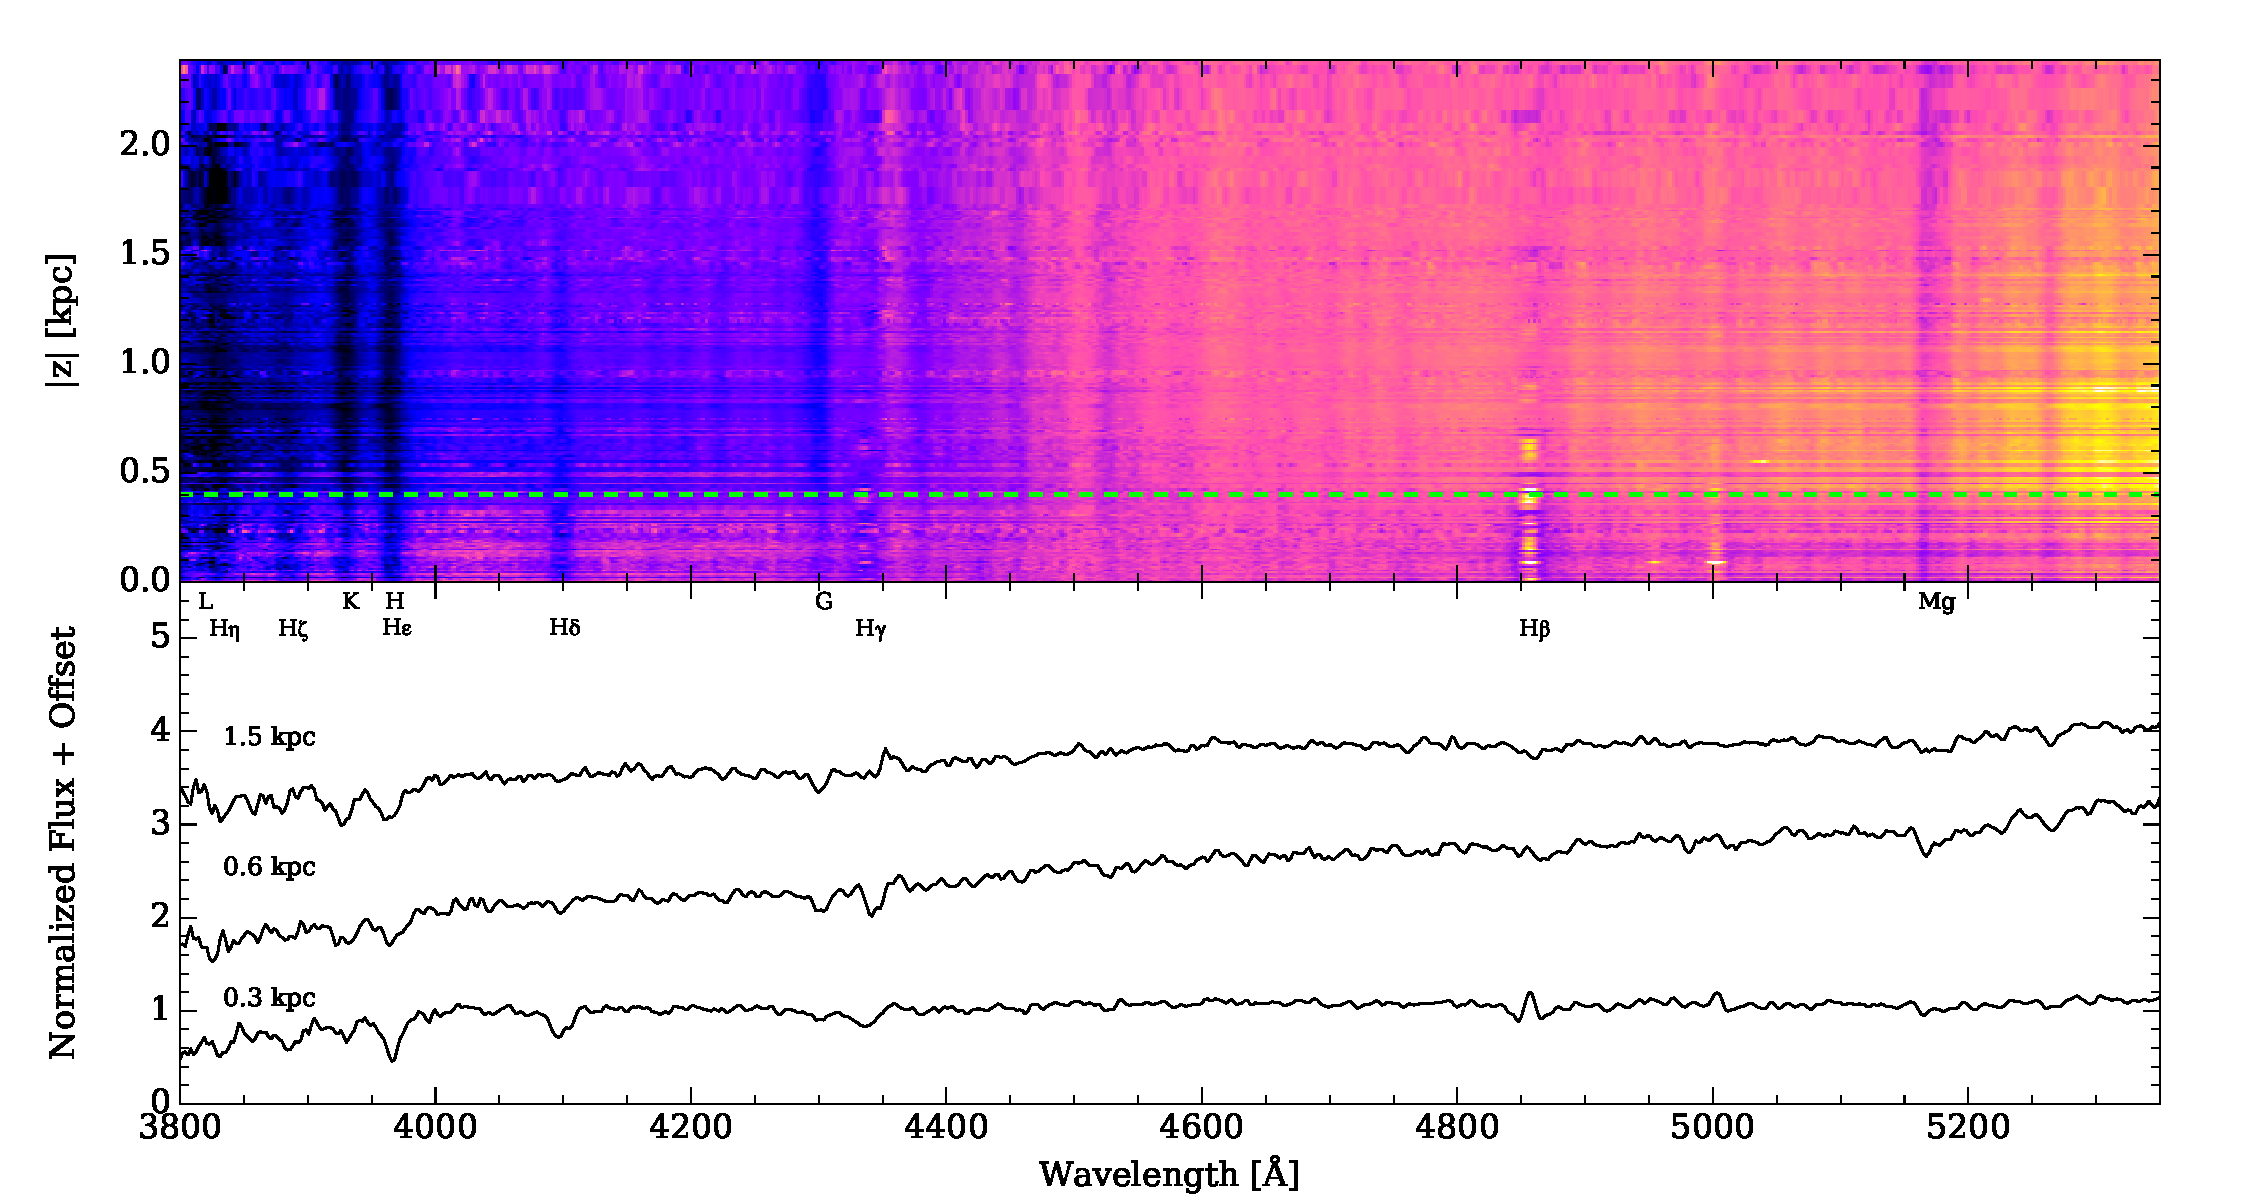
\includegraphics[width=\textwidth]{891_1/figs/mab_data_stack.pdf}
  \caption[Heating signature in NGC 891 \GP
  data]{\label{891_1:fig:mab_data}\fixspacing Same as Figure
    \ref{891_1:fig:MW_heating}, but for the \GP data from NGC 891. Top:
    Normalized galaxy spectra at different heights, color-coded by
    intensity (see text for a description of how this image was
    made). The horizontal line marks the age break at \val{0.4}{kpc}
    described for Figure \ref{891_1:fig:D4000_cuts}. Bottom: Representative
    spectra at three different heights (labeled). Prominent spectral
    features are labeled at the boundary between the two panels.}
\end{figure*}

\subsection{Vertical Trends}

The almost perfectly edge-on nature of NGC 891 allows unambiguous
determination of vertical trends in our spectra. Figure
\ref{891_1:fig:mab_data} presents our data for direct comparison to Figure
\ref{891_1:fig:MW_heating}. This was made by sorting spectra from all
apertures by height, regardless of radius, and then interpolating them
onto a regular grid to form a linear scale in kpc. The grid spacing (8
pc) was chosen for cosmetic reasons to keep the interpolation from
being apparent except at the largest heights. As with the model
spectra in Figure \ref{891_1:fig:MW_heating}, the individual spectra were
first normalized by their mean value.

% Apertures for spectra in \ref{fig:mab_data}
% 0.3 kpc - P6.12
% 0.6 kpc - P3.32
% 1.5 kpc - P6.33

The transition from young, Balmer-dominated spectra to
old, metal-dominated spectra is clear at \val{0.4}{kpc}, as
highlighted by the example spectra. At \val{0.3}{kpc} Balmer
absorption dominates, but a larger heights strong Ca H\&K and G band
absorption indicate the presence of older populations.  The amazing
match between Figures \ref{891_1:fig:MW_heating} and \ref{891_1:fig:mab_data} is
even more remarkable given that the MW heating model used in Figure
\ref{891_1:fig:MW_heating} includes no information about NGC 891 and is
simply tuned to observations from the Solar Cylinder.

This first-blush qualitative comparison has visceral appeal, and
demonstrates the vertical trends in stellar populations seen in the MW
(as described in \S\ref{891_1:sec:introduction}) are manifest in NGC
891. However, the comparison lacks quantitative rigor.  Our primary
interest is to quantify the comparison and determine to what extent
these trends also depend on radius. In particular, precise location of
a sharp vertical transition from Balmer-line to metal-line dominated
spectra can be used to calibrate how disk stars are vertically
stratified in phase space as a function of age and radial
location. This in turn can be interpreted in terms of time-scales for
dynamical heating or gas-cooling models, and the extent to which
vertical age gradients in spiral disks are ubiquitous and
quantitatively similar or distinct.

Disentangling age from metallicity, and metallicity from abundance is
fraught with degeneracies, particularly in complex stellar populations
observed in integrated star-light. In an edge-on galaxy like NGC 891,
there is the additional complication of projection effects compounded
with extinction that is patchy, but also changes broadly with height
and radius. Paper II undertakes to model all of these complexities,
but here we are interested in using simple spectral indices, the
measured value of which are model-independent and insensitive to
redenning. These indices allow us to we probe for vertical {\it age}
transitions and their radial trends while at the same time bounding
(providing priors on) the age and metallicity of the more complicated
modeling we later undertake.

\subsection{Spectral Indices}
\label{891_1:sec:indices}

\subsubsection{Definitions}
\label{891_1:sec:index_defn}

We focus our attention on the spectral indices defined in Table
\ref{891_1:tab:indices}. The first two entries have primary sensitivity to
age, while the remainder are primarily sensitive to metallicity, and,
in combination, to abundance. Because the age-sensitive indices have
varying degrees of dependence on metallicity and vice versa, index
combinations are required to disentangle these effects, as well
established in the literature, particularly for older stellar
populations, as we cite in what follows.

The strength of Balmer absorption has long been used as a mostly
metallicity-insensitive measure of population age because it depends
primarily on the main-sequence turn off temperature instead of the red
giant branch temperature. In other words, strong Balmer absorption is
produced by young, hot main-sequence stars with lifetimes of
$<\val{100}{Myr}$, regardless of metal content. \citet{Worthey97} find
that of the Balmer absorption lines \HB is the least sensitive to
metallicity (due to a lack of adjacent metal lines that impact the
continuum) and, given its relative strength, is the most sensitive to
age.  However, contamination from nebular emission is problematic,
with increasing intensity for the lower-order Balmer lines.  All of
our spectra show strong signs of \Ha emission and in some apertures
Balmer lines have negative equivalent widths as high as \Hg.  The
traditional trade between age sensitivity (i.e., \emph{insensitivity}
to metallicity variations) and systematics due to nebular emission, is
to use \Hda \citep{Worthey97} as an age indicator, which in fact has
long been used in extragalactic studies of mixed stellar populations
\citep[e.g.,][]{Couch87}. In Paper II we develop a model for Balmer
emission and find that applying an emission correction correction
shifts \Hda by \val{-0.4\pm 0.3}{\AA}, which is roughly 10\% of the
dynamic range in \Hda across the age transition found in
\S\ref{891_1:sec:age_grad}.

The break at \val{4000}{\AA} can also be used to estimate the age of
stellar populations, albeit with a larger sensitivity to
metallicity. This break is caused by an increase in opacity resulting
from ionization of metal lines; young stars are hot enough to put
metals into high ionization states and the thus the total opacity is
low. As temperature decreases more of the metals occupy lower
ionization states that are suitable for absorption and the opacity
increases. Beyond a certain limit very cool stars (i.e., M stars) are
unable to even singly ionize the neutral atoms and the amplitude of
the break decreases. Thus the \val{4000}{\AA} break traces population
age (specifically related to the temperature of the red giant branch),
but also depends on the population metallicity, although not as
strongly \citep[see][and Figure \ref{891_1:fig:D4000_cuts} here]{Bruzual83}.
The metal line that contributes most to the \val{4000}{\AA} break is
Ca K at \val{3933}{\AA}, which causes the magnitude of the break to
also exhibit a weak dependence on abundance. To measure the
\val{4000}{\AA} break we use the narrower-band definition of
\citet{Balogh99} primarily because our flux calibration deteriorates
blueward of \val{3800}{\AA} (Figure \ref{891_1:fig:sky_flux_comp}), and we
adopt the nomenclature, $D_n(4000)$, of \citet{Kauffmann03}.

We also define composite indices to determine metallicity and
$\alpha$-enhancement in our populations. In particular,
\citet{Thomas03} find that 
\begin{equation}
\mathrm{[MgFe]} = \sqrt{\mathrm{Mg
    \emph{b}}(0.72\times\mathrm{Fe}_{5270} +
  0.28\times\mathrm{Fe}_{5335})}
\end{equation}
is almost totally insensitive to changes in abundance and is therefore
a good tracer of the total metallicity in a stellar population. They
also note that, when plotted against Mg$b$, Fe$_{5270}$, Fe$_{5335}$,
and Fe$_{5408}$ are all fairly sensitive to changes in abundance. We
choose to use $\left<\mathrm{Fe}\right>$ =
(Fe$_{5270}$+Fe$_{5335}$)/2, because these two Fe indices are slightly
better calibrated than Fe$_{5408}$ \citep{Thomas03} and have been have
been used in other important studies
\citep[e.g.,][]{Trager05,Trager08,Trager09}.

The reported ``indices'' are equivalent widths defined as
\begin{equation}
  EW = \left(1 - \frac{F_I}{F_C}\right)\Delta_{\lambda},
\end{equation}
where $F_I$ and $F_C$ are the average fluxes in the index and
continuum bands, respectively and $\Delta_{\lambda}$ is the width of
the index bandpass defined in Table \ref{891_1:tab:indices}. The value of
$F_C$ is computed by linearly interpolating the flux computed in the
red and blue continuum bands to the center of the index band. In the
case of $D_n(4000)$ the reported value is simply the ratio of the
average flux in the red continuum band to the average flux in the blue
continuum band. Table \ref{891_1:tab:index_res} reports our measured values
for all appertures defined in Table \ref{891_1:tab:data_ap}.

Recognizing the wisdom of \citet{Balogh99} we caution that the
absolute values of our measured indices do not correspond to physical
quantities. The specific conditions of our data (e.g., spectral
resolution, sampling, signal-to-noise, etc.) can and will affect the
derived index values and the reader is warned away from comparing our
results in an absolute sense to those of other studies unless they are
careful to match to our spectral sampling and resolution as described
in Section \ref{891_1:sec:obs}.

\begin{deluxetable}{lccccccc}
\tablewidth{0pt}
\tablecaption{Spectral Index Definitions}
\tablehead{
%  & \multicolumn{6}{c}{Bandpass (\AA)}\\
%  & \multicolumn{6}{\hline}\\
  \colhead{Index} &
  \multicolumn{2}{c}{On-Band} &
  \multicolumn{2}{c}{Blue Continuum} &
  \multicolumn{2}{c}{Red Continuum} \\
  \colhead{Name} &
  \colhead{Center} &
  \colhead{Width} &
  \colhead{Center} &
  \colhead{Width} &
  \colhead{Center} &
  \colhead{Width}\\
  \colhead{} &
  \colhead{(\AA)} &
  \colhead{(\AA)} &
  \colhead{(\AA)} &
  \colhead{(\AA)} &
  \colhead{(\AA)} &
  \colhead{(\AA)}}
\startdata
$D_n(4000)$ & - & - & 3900 & 100 & 4050 & 100 \\
H$\delta_A$ & 4103.9 & 38.8 & 4060.7 & 38.1 & 4144.8 & 32.5 \\
%H$\gamma_A$ & 4341.6 & 43.8 & 4301.6 & 36.3 & 4393.5 & 52.5 \\
%\HB         & 4862.3 & 28.8 & 4837.9 & 20.0 & 4884.1 & 15.0 \\
Mg\emph{b} & 5176.4 & 32.5 & 5152.0 & 18.8 & 5198.9 & 15.0 \\
Fe$_{5270}$  & 5265.7 & 40.0 & 5240.7 & 15.0 & 5301.9 & 32.5 \\
Fe$_{5335}$  & 5332.1 & 40.0 & 5310.3 & 11.3 & 5358.4 & 10.0
\enddata
\label{891_1:tab:indices}
\end{deluxetable}

\clearpage
\begin{deluxetable}{ccccccccc}
\tablewidth{0pt}
\tablecaption{NGC 891 Index Measurements}
\tablehead{
    \colhead{Pointing} &
    \colhead{Aperture} &
    \colhead{$r_\mathrm{proj}$} &
    \colhead{$z$} &
    \colhead{$D_n4000$} &
    \colhead{$H\delta_A$} &
    \colhead{Mg$b$} &
    \colhead{$\left<\mathrm{Fe}\right>$} &
    \colhead{[MgFe]}\\
    \colhead{Number} &
    \colhead{Number} &
    \colhead{(kpc)} &
    \colhead{(kpc)} &
    \colhead{} &
    \colhead{(\AA)} &
    \colhead{(\AA)} &
    \colhead{(\AA)} &
    \colhead{(\AA)}
}
\startdata
 1 &  1 & 4.44 & -0.12 & 1.64 $\pm$ 0.04 & 5.91 $\pm$ 0.85 & 1.99 $\pm$ 0.47 & 0.76 $\pm$ 0.37 & 1.36 $\pm$ 0.32\\
 1 &  2 & 5.26 & -0.09 & 1.20 $\pm$ 0.02 & 4.20 $\pm$ 0.78 & 1.43 $\pm$ 0.56 & 0.95 $\pm$ 0.46 & 1.35 $\pm$ 0.35\\
  %%  1 &  3 & 4.16 & 0.02 & 1.37 $\pm$ 0.03 & 2.63 $\pm$ 1.01 & 2.27 $\pm$ 0.56 & 1.54 $\pm$ 0.40 & 1.91 $\pm$ 0.34\\
  %%  1 &  4 & 4.76 & 0.04 & 1.29 $\pm$ 0.02 & 4.64 $\pm$ 0.62 & 2.09 $\pm$ 0.49 & 1.07 $\pm$ 0.40 & 1.51 $\pm$ 0.33\\
  %%  1 &  5 & 5.52 & 0.07 & 1.11 $\pm$ 0.05 & 7.10 $\pm$ 1.77 & 2.49 $\pm$ 0.95 & -0.16 $\pm$ 0.92 &  nan $\pm$  nan\\
  %%  1 &  6 & 4.67 & 0.21 & 1.29 $\pm$ 0.02 & 5.19 $\pm$ 0.71 & 1.73 $\pm$ 0.52 & 0.81 $\pm$ 0.41 & 1.03 $\pm$ 0.39\\
  %%  1 &  7 & 5.51 & 0.24 & 1.32 $\pm$ 0.05 & 5.38 $\pm$ 1.59 & 1.66 $\pm$ 0.94 & 0.67 $\pm$ 0.91 & 0.86 $\pm$ 0.85\\
  %%  1 &  8 & 4.47 & 0.41 & 1.17 $\pm$ 0.02 & 6.28 $\pm$ 0.64 & 1.52 $\pm$ 0.49 & 1.46 $\pm$ 0.39 & 1.65 $\pm$ 0.32\\
  %%  1 &  9 & 5.24 & 0.44 & 1.51 $\pm$ 0.03 & 1.90 $\pm$ 0.85 & 1.89 $\pm$ 0.39 & 1.40 $\pm$ 0.28 & 1.77 $\pm$ 0.23\\
  %%  1 & 10 & 5.68 & 0.46 & 1.63 $\pm$ 0.05 & 2.02 $\pm$ 1.25 & 1.89 $\pm$ 0.54 & 1.60 $\pm$ 0.45 & 1.95 $\pm$ 0.36\\
  %%  1 & 11 & 4.61 & 0.63 & 1.61 $\pm$ 0.03 & 2.30 $\pm$ 0.71 & 1.86 $\pm$ 0.35 & 1.52 $\pm$ 0.30 & 1.79 $\pm$ 0.22\\
  %%  1 & 12 & 5.45 & 0.67 & 1.84 $\pm$ 0.04 & 2.08 $\pm$ 0.84 & 1.85 $\pm$ 0.48 & 1.46 $\pm$ 0.33 & 1.76 $\pm$ 0.29\\
  %%  1 & 13 & 5.67 & 0.68 & 1.84 $\pm$ 0.05 & 2.40 $\pm$ 0.83 & 2.11 $\pm$ 0.40 & 1.62 $\pm$ 0.36 & 1.90 $\pm$ 0.26\\
  %%  1 & 14 & 4.22 & 0.87 & 1.71 $\pm$ 0.04 & 1.50 $\pm$ 0.78 & 1.85 $\pm$ 0.36 & 1.37 $\pm$ 0.37 & 1.65 $\pm$ 0.25\\
  %%  1 & 15 & 4.62 & 0.89 & 1.72 $\pm$ 0.04 & 0.81 $\pm$ 0.90 & 2.20 $\pm$ 0.46 & 1.50 $\pm$ 0.45 & 1.95 $\pm$ 0.30\\
  %%  1 & 16 & 4.89 & 0.90 & 1.75 $\pm$ 0.04 & 1.56 $\pm$ 0.96 & 2.46 $\pm$ 0.55 & 1.33 $\pm$ 0.54 & 1.95 $\pm$ 0.38\\
  %%  1 & 17 & 5.16 & 0.91 & 1.74 $\pm$ 0.04 & 1.61 $\pm$ 0.83 & 2.48 $\pm$ 0.52 & 1.52 $\pm$ 0.50 & 2.06 $\pm$ 0.34\\
  %%  1 & 18 & 5.43 & 0.92 & 1.58 $\pm$ 0.04 & 1.19 $\pm$ 0.75 & 1.90 $\pm$ 0.47 & 1.31 $\pm$ 0.42 & 1.66 $\pm$ 0.29\\
  %%  1 & 19 & 5.69 & 0.94 & 1.75 $\pm$ 0.04 & 0.08 $\pm$ 0.90 & 1.92 $\pm$ 0.51 & 1.79 $\pm$ 0.50 & 1.96 $\pm$ 0.33\\
  %%  1 & 20 & 4.07 & 1.14 & 1.62 $\pm$ 0.04 & 1.59 $\pm$ 0.94 & 2.48 $\pm$ 0.55 & 1.13 $\pm$ 0.54 & 1.79 $\pm$ 0.39\\
  %%  1 & 21 & 4.34 & 1.15 & 1.63 $\pm$ 0.03 & 0.92 $\pm$ 0.82 & 2.23 $\pm$ 0.36 & 1.63 $\pm$ 0.34 & 2.06 $\pm$ 0.24\\
  %%  1 & 22 & 4.61 & 1.16 & 1.65 $\pm$ 0.04 & 2.07 $\pm$ 0.98 & 2.33 $\pm$ 0.45 & 1.37 $\pm$ 0.47 & 1.89 $\pm$ 0.30\\
  %%  1 & 23 & 4.88 & 1.17 & 1.57 $\pm$ 0.03 & 0.86 $\pm$ 0.71 & 2.25 $\pm$ 0.33 & 1.45 $\pm$ 0.38 & 1.87 $\pm$ 0.26\\
  %%  1 & 24 & 5.15 & 1.18 & 1.60 $\pm$ 0.03 & 1.33 $\pm$ 0.72 & 2.41 $\pm$ 0.52 & 2.00 $\pm$ 0.48 & 2.31 $\pm$ 0.34\\
  %%  1 & 25 & 5.55 & 1.20 & 1.56 $\pm$ 0.03 & 0.10 $\pm$ 0.85 & 2.15 $\pm$ 0.47 & 1.29 $\pm$ 0.48 & 1.84 $\pm$ 0.32\\
  %%  1 & 26 & 4.06 & 1.40 & 1.63 $\pm$ 0.03 & 0.53 $\pm$ 0.67 & 1.93 $\pm$ 0.41 & 1.53 $\pm$ 0.36 & 1.77 $\pm$ 0.26\\
  %%  1 & 27 & 4.33 & 1.42 & 1.54 $\pm$ 0.03 & 0.54 $\pm$ 0.72 & 2.20 $\pm$ 0.39 & 1.43 $\pm$ 0.38 & 1.86 $\pm$ 0.26\\
  %%  1 & 28 & 4.60 & 1.43 & 1.55 $\pm$ 0.03 & 0.67 $\pm$ 0.71 & 2.22 $\pm$ 0.49 & 1.64 $\pm$ 0.48 & 2.00 $\pm$ 0.32\\
  %%  1 & 29 & 5.00 & 1.44 & 1.50 $\pm$ 0.03 & 0.69 $\pm$ 0.75 & 2.09 $\pm$ 0.48 & 1.58 $\pm$ 0.48 & 1.91 $\pm$ 0.32\\
  %%  1 & 30 & 5.54 & 1.47 & 1.42 $\pm$ 0.04 & -1.41 $\pm$ 1.21 & 1.72 $\pm$ 0.73 & 0.53 $\pm$ 0.79 & 1.10 $\pm$ 0.58\\
  %%  1 & 31 & 4.04 & 1.71 & 1.54 $\pm$ 0.03 & 0.18 $\pm$ 0.79 & 2.93 $\pm$ 0.39 & 1.20 $\pm$ 0.33 & 1.96 $\pm$ 0.27\\
  %%  1 & 32 & 4.37 & 1.72 & 1.52 $\pm$ 0.03 & 0.49 $\pm$ 0.82 & 2.24 $\pm$ 0.44 & 1.36 $\pm$ 0.37 & 1.88 $\pm$ 0.28\\
  %%  1 & 33 & 4.85 & 1.75 & 1.65 $\pm$ 0.03 & 1.01 $\pm$ 0.76 & 2.42 $\pm$ 0.48 & 1.27 $\pm$ 0.33 & 1.79 $\pm$ 0.28\\
  %%  1 & 34 & 5.50 & 1.77 & 1.87 $\pm$ 0.05 & -0.46 $\pm$ 0.99 & 1.71 $\pm$ 0.62 & 1.85 $\pm$ 0.48 & 1.82 $\pm$ 0.40\\
  %%  1 & 35 & 4.19 & 2.04 & 1.54 $\pm$ 0.03 & -0.83 $\pm$ 0.90 & 2.95 $\pm$ 0.40 & 1.20 $\pm$ 0.32 & 2.09 $\pm$ 0.27\\
  %%  1 & 36 & 5.16 & 2.08 & 1.55 $\pm$ 0.03 & 0.82 $\pm$ 0.90 & 2.47 $\pm$ 0.50 & 1.26 $\pm$ 0.39 & 1.92 $\pm$ 0.32\\
  %%  1 & 37 & 4.82 & 2.39 & 1.28 $\pm$ 0.02 & -0.50 $\pm$ 0.93 & 1.76 $\pm$ 0.48 & 1.24 $\pm$ 0.42 & 1.56 $\pm$ 0.31\\
 2 &  1 & 1.27 & -0.17 & 1.41 $\pm$ 0.08 & -0.71 $\pm$ 2.54 & 2.95 $\pm$ 1.02 & 1.68 $\pm$ 0.78 & 2.22 $\pm$ 0.64\\
 2 &  2 & 1.26 & -0.02 & 1.10 $\pm$ 0.04 & 7.57 $\pm$ 1.44 & 1.47 $\pm$ 1.06 & 0.65 $\pm$ 0.68 & 1.06 $\pm$ 0.63\\
  %%  2 &  3 & 1.26 & 0.15 & 1.25 $\pm$ 0.04 & 6.53 $\pm$ 1.07 & 0.83 $\pm$ 0.75 & -0.01 $\pm$ 0.69 &  nan $\pm$  nan\\
  %%  2 &  4 & 1.25 & 0.35 & 1.45 $\pm$ 0.02 & 2.99 $\pm$ 0.64 & 1.91 $\pm$ 0.36 & 1.65 $\pm$ 0.38 & 1.86 $\pm$ 0.25\\
  %%  2 &  5 & 0.69 & 0.55 & 1.68 $\pm$ 0.03 & 0.39 $\pm$ 0.72 & 1.95 $\pm$ 0.44 & 1.53 $\pm$ 0.39 & 1.84 $\pm$ 0.29\\
  %%  2 &  6 & 1.35 & 0.58 & 1.81 $\pm$ 0.04 & 1.59 $\pm$ 0.64 & 2.22 $\pm$ 0.33 & 1.71 $\pm$ 0.29 & 2.09 $\pm$ 0.21\\
  %%  2 &  7 & 1.90 & 0.60 & 1.83 $\pm$ 0.05 & 1.05 $\pm$ 1.10 & 2.19 $\pm$ 0.49 & 1.39 $\pm$ 0.39 & 1.86 $\pm$ 0.31\\
  %%  2 &  8 & 0.42 & 0.79 & 1.88 $\pm$ 0.03 & 0.21 $\pm$ 0.61 & 2.26 $\pm$ 0.19 & 1.56 $\pm$ 0.15 & 1.94 $\pm$ 0.12\\
  %%  2 &  9 & 0.69 & 0.81 & 1.76 $\pm$ 0.03 & 1.16 $\pm$ 0.51 & 1.21 $\pm$ 0.24 & 0.67 $\pm$ 0.19 & 1.08 $\pm$ 0.14\\
  %%  2 & 10 & 0.96 & 0.82 & 1.81 $\pm$ 0.02 & 0.66 $\pm$ 0.45 & 2.09 $\pm$ 0.24 & 1.24 $\pm$ 0.21 & 1.73 $\pm$ 0.16\\
  %%  2 & 11 & 1.23 & 0.83 & 1.84 $\pm$ 0.03 & 1.09 $\pm$ 0.69 & 2.12 $\pm$ 0.35 & 1.24 $\pm$ 0.25 & 1.72 $\pm$ 0.21\\
  %%  2 & 12 & 1.49 & 0.84 & 1.75 $\pm$ 0.03 & 0.42 $\pm$ 0.65 & 1.88 $\pm$ 0.24 & 1.50 $\pm$ 0.24 & 1.81 $\pm$ 0.16\\
  %%  2 & 13 & 1.76 & 0.85 & 1.67 $\pm$ 0.04 & 0.14 $\pm$ 0.82 & 2.45 $\pm$ 0.24 & 1.54 $\pm$ 0.22 & 1.97 $\pm$ 0.17\\
  %%  2 & 14 & 2.03 & 0.86 & 1.67 $\pm$ 0.04 & 1.51 $\pm$ 1.01 & 1.74 $\pm$ 0.38 & 1.09 $\pm$ 0.27 & 1.56 $\pm$ 0.22\\
  %%  2 & 15 & 0.41 & 1.06 & 1.76 $\pm$ 0.03 & 0.35 $\pm$ 0.60 & 2.04 $\pm$ 0.27 & 1.59 $\pm$ 0.24 & 1.88 $\pm$ 0.18\\
  %%  2 & 16 & 0.68 & 1.07 & 1.72 $\pm$ 0.03 & 0.72 $\pm$ 0.57 & 1.59 $\pm$ 0.37 & 1.06 $\pm$ 0.24 & 1.38 $\pm$ 0.20\\
  %%  2 & 17 & 0.95 & 1.08 & 1.68 $\pm$ 0.02 & -0.21 $\pm$ 0.56 & 2.18 $\pm$ 0.29 & 1.21 $\pm$ 0.29 & 1.76 $\pm$ 0.20\\
  %%  2 & 18 & 1.21 & 1.10 & 1.71 $\pm$ 0.03 & 0.89 $\pm$ 0.53 & 2.06 $\pm$ 0.29 & 1.15 $\pm$ 0.23 & 1.64 $\pm$ 0.17\\
  %%  2 & 19 & 1.48 & 1.11 & 1.69 $\pm$ 0.03 & 1.31 $\pm$ 0.68 & 2.04 $\pm$ 0.33 & 1.29 $\pm$ 0.24 & 1.76 $\pm$ 0.19\\
  %%  2 & 20 & 1.75 & 1.12 & 1.68 $\pm$ 0.03 & -0.04 $\pm$ 0.80 & 2.61 $\pm$ 0.35 & 1.58 $\pm$ 0.32 & 2.14 $\pm$ 0.23\\
  %%  2 & 21 & 2.02 & 1.13 & 1.53 $\pm$ 0.04 & 1.09 $\pm$ 0.78 & 1.76 $\pm$ 0.42 & 0.37 $\pm$ 0.38 & 1.00 $\pm$ 0.35\\
  %%  2 & 22 & 0.40 & 1.33 & 1.69 $\pm$ 0.03 & -0.22 $\pm$ 0.81 & 1.87 $\pm$ 0.36 & 1.35 $\pm$ 0.39 & 1.67 $\pm$ 0.28\\
  %%  2 & 23 & 0.67 & 1.34 & 1.68 $\pm$ 0.03 & 0.58 $\pm$ 0.65 & 2.07 $\pm$ 0.37 & 1.07 $\pm$ 0.27 & 1.51 $\pm$ 0.25\\
  %%  2 & 24 & 0.93 & 1.35 & 1.65 $\pm$ 0.02 & 0.05 $\pm$ 0.73 & 1.85 $\pm$ 0.34 & 1.49 $\pm$ 0.35 & 1.73 $\pm$ 0.23\\
  %%  2 & 25 & 1.20 & 1.36 & 1.60 $\pm$ 0.03 & -0.26 $\pm$ 0.65 & 2.24 $\pm$ 0.48 & 1.57 $\pm$ 0.44 & 1.95 $\pm$ 0.34\\
  %%  2 & 26 & 1.47 & 1.38 & 1.65 $\pm$ 0.03 & 0.14 $\pm$ 0.69 & 2.28 $\pm$ 0.46 & 1.50 $\pm$ 0.38 & 1.86 $\pm$ 0.30\\
  %%  2 & 27 & 1.74 & 1.39 & 1.60 $\pm$ 0.04 & 0.61 $\pm$ 0.91 & 2.19 $\pm$ 0.44 & 1.30 $\pm$ 0.45 & 1.81 $\pm$ 0.31\\
  %%  2 & 28 & 2.01 & 1.40 & 1.56 $\pm$ 0.05 & 0.70 $\pm$ 0.96 & 1.85 $\pm$ 0.78 & 1.51 $\pm$ 0.56 & 1.65 $\pm$ 0.50\\
  %%  2 & 29 & 0.38 & 1.64 & 1.58 $\pm$ 0.04 & -0.92 $\pm$ 0.97 & 1.96 $\pm$ 0.41 & 1.28 $\pm$ 0.43 & 1.75 $\pm$ 0.28\\
  %%  2 & 30 & 0.70 & 1.65 & 1.55 $\pm$ 0.03 & -0.55 $\pm$ 0.79 & 1.88 $\pm$ 0.54 & 0.91 $\pm$ 0.38 & 1.38 $\pm$ 0.31\\
  %%  2 & 31 & 1.03 & 1.67 & 1.69 $\pm$ 0.04 & 0.42 $\pm$ 0.84 & 1.64 $\pm$ 0.63 & 0.49 $\pm$ 0.53 & 1.09 $\pm$ 0.41\\
  %%  2 & 32 & 1.35 & 1.68 & 1.60 $\pm$ 0.04 & 0.81 $\pm$ 0.90 & 1.81 $\pm$ 0.48 & 0.87 $\pm$ 0.34 & 1.39 $\pm$ 0.32\\
  %%  2 & 33 & 1.68 & 1.69 & 1.66 $\pm$ 0.04 & 2.20 $\pm$ 1.04 & 1.88 $\pm$ 0.58 & 1.16 $\pm$ 0.43 & 1.64 $\pm$ 0.36\\
  %%  2 & 34 & 2.00 & 1.71 & 1.63 $\pm$ 0.04 & 0.73 $\pm$ 0.89 & 1.45 $\pm$ 0.54 & 0.56 $\pm$ 0.47 & 0.98 $\pm$ 0.40\\
  %%  2 & 35 & 0.36 & 1.96 & 1.51 $\pm$ 0.04 & -0.46 $\pm$ 1.03 & -0.20 $\pm$ 0.51 & -0.34 $\pm$ 0.41 & 0.26 $\pm$ 0.36\\
  %%  2 & 36 & 1.18 & 2.00 & 1.53 $\pm$ 0.03 & 0.45 $\pm$ 0.78 & 1.80 $\pm$ 0.43 & 0.88 $\pm$ 0.35 & 1.32 $\pm$ 0.28\\
  %%  2 & 37 & 1.99 & 2.03 & 1.44 $\pm$ 0.06 & 0.37 $\pm$ 1.58 & 0.55 $\pm$ 1.16 & 1.30 $\pm$ 0.72 & 0.94 $\pm$ 1.02\\
  %%  2 & 38 & 1.16 & 2.32 & 1.35 $\pm$ 0.03 & 0.25 $\pm$ 0.95 & 1.60 $\pm$ 0.57 & 0.80 $\pm$ 0.48 & 1.22 $\pm$ 0.37\\
 3 &  1 & -6.31 & -0.17 & 1.52 $\pm$ 0.02 & 4.36 $\pm$ 0.50 & 1.42 $\pm$ 0.38 & 1.30 $\pm$ 0.30 & 1.43 $\pm$ 0.24\\
 3 &  2 & -5.98 & -0.16 & 1.29 $\pm$ 0.02 & 4.49 $\pm$ 0.70 & 1.34 $\pm$ 0.49 & 1.14 $\pm$ 0.36 & 1.36 $\pm$ 0.30\\
  %%  3 &  3 & -5.76 & -0.15 & 1.30 $\pm$ 0.02 & 3.37 $\pm$ 0.72 & 1.89 $\pm$ 0.52 & 0.78 $\pm$ 0.45 & 1.31 $\pm$ 0.34\\
  %%  3 &  4 & -5.43 & -0.14 & 1.18 $\pm$ 0.01 & 3.06 $\pm$ 0.57 & 2.07 $\pm$ 0.51 & 1.22 $\pm$ 0.42 & 1.70 $\pm$ 0.32\\
  %%  3 &  5 & -5.05 & -0.12 & 1.18 $\pm$ 0.01 & 5.42 $\pm$ 0.56 & 1.76 $\pm$ 0.49 & 1.33 $\pm$ 0.37 & 1.53 $\pm$ 0.29\\
  %%  3 &  6 & -6.39 & -0.03 & 1.16 $\pm$ 0.01 & 5.14 $\pm$ 0.40 & 1.30 $\pm$ 0.39 & 0.93 $\pm$ 0.35 & 1.13 $\pm$ 0.26\\
  %%  3 &  7 & -6.13 & -0.01 & 1.16 $\pm$ 0.01 & 4.03 $\pm$ 0.47 & 0.88 $\pm$ 0.46 & 0.57 $\pm$ 0.36 & 0.80 $\pm$ 0.28\\
  %%  3 &  8 & -5.97 & -0.01 & 1.13 $\pm$ 0.01 & 3.85 $\pm$ 0.49 & 0.58 $\pm$ 0.35 & 0.33 $\pm$ 0.31 & 0.55 $\pm$ 0.23\\
  %%  3 &  9 & -5.80 & 0.00 & 1.09 $\pm$ 0.01 & 4.46 $\pm$ 0.50 & 1.36 $\pm$ 0.46 & 0.81 $\pm$ 0.40 & 1.14 $\pm$ 0.30\\
  %%  3 & 10 & -5.63 & 0.01 & 1.19 $\pm$ 0.02 & 3.11 $\pm$ 0.81 & 1.30 $\pm$ 0.46 & 0.84 $\pm$ 0.43 & 1.09 $\pm$ 0.32\\
  %%  3 & 11 & -5.46 & 0.01 & 1.21 $\pm$ 0.01 & 4.54 $\pm$ 0.46 & 1.75 $\pm$ 0.35 & 0.92 $\pm$ 0.32 & 1.35 $\pm$ 0.24\\
  %%  3 & 12 & -5.20 & 0.03 & 1.19 $\pm$ 0.01 & 4.70 $\pm$ 0.46 & 1.79 $\pm$ 0.34 & 0.54 $\pm$ 0.27 & 1.09 $\pm$ 0.24\\
  %%  3 & 13 & -4.95 & 0.04 & 1.20 $\pm$ 0.01 & 3.63 $\pm$ 0.63 & 1.28 $\pm$ 0.57 & 0.56 $\pm$ 0.43 & 0.91 $\pm$ 0.37\\
  %%  3 & 14 & -6.48 & 0.14 & 1.26 $\pm$ 0.01 & 5.66 $\pm$ 0.41 & 0.94 $\pm$ 0.43 & 0.95 $\pm$ 0.38 & 1.07 $\pm$ 0.29\\
  %%  3 & 15 & -6.31 & 0.15 & 1.17 $\pm$ 0.01 & 5.07 $\pm$ 0.42 & 1.18 $\pm$ 0.33 & 0.86 $\pm$ 0.27 & 1.14 $\pm$ 0.21\\
  %%  3 & 16 & -6.14 & 0.15 & 1.21 $\pm$ 0.01 & 4.88 $\pm$ 0.50 & 0.99 $\pm$ 0.36 & 0.74 $\pm$ 0.31 & 0.82 $\pm$ 0.24\\
  %%  3 & 17 & -5.89 & 0.17 & 1.15 $\pm$ 0.01 & 4.11 $\pm$ 0.51 & 1.04 $\pm$ 0.40 & 0.68 $\pm$ 0.33 & 0.92 $\pm$ 0.25\\
  %%  3 & 18 & -5.55 & 0.18 & 1.21 $\pm$ 0.01 & 4.16 $\pm$ 0.55 & 1.17 $\pm$ 0.36 & 0.66 $\pm$ 0.28 & 0.99 $\pm$ 0.22\\
  %%  3 & 19 & -5.29 & 0.19 & 1.26 $\pm$ 0.02 & 1.92 $\pm$ 0.84 & 0.90 $\pm$ 0.54 & 0.96 $\pm$ 0.36 & 1.02 $\pm$ 0.35\\
  %%  3 & 20 & -5.04 & 0.20 & 1.30 $\pm$ 0.02 & 3.18 $\pm$ 0.58 & 1.28 $\pm$ 0.33 & 1.10 $\pm$ 0.28 & 1.27 $\pm$ 0.21\\
  %%  3 & 21 & -6.50 & 0.35 & 1.28 $\pm$ 0.02 & 4.71 $\pm$ 0.71 & 1.61 $\pm$ 0.35 & 1.09 $\pm$ 0.31 & 1.35 $\pm$ 0.23\\
  %%  3 & 22 & -6.28 & 0.36 & 1.25 $\pm$ 0.02 & 1.06 $\pm$ 0.93 & 1.33 $\pm$ 0.57 & 1.04 $\pm$ 0.44 & 1.24 $\pm$ 0.35\\
  %%  3 & 23 & -6.06 & 0.37 & 1.22 $\pm$ 0.01 & 2.99 $\pm$ 0.57 & 1.96 $\pm$ 0.36 & 1.10 $\pm$ 0.29 & 1.55 $\pm$ 0.23\\
  %%  3 & 24 & -5.84 & 0.38 & 1.20 $\pm$ 0.01 & 2.99 $\pm$ 0.55 & 1.71 $\pm$ 0.29 & 1.05 $\pm$ 0.26 & 1.43 $\pm$ 0.19\\
  %%  3 & 25 & -5.51 & 0.39 & 1.24 $\pm$ 0.01 & 2.28 $\pm$ 0.44 & 1.61 $\pm$ 0.33 & 1.09 $\pm$ 0.24 & 1.27 $\pm$ 0.20\\
  %%  3 & 26 & -5.18 & 0.40 & 1.37 $\pm$ 0.02 & 2.30 $\pm$ 0.55 & 2.04 $\pm$ 0.38 & 1.06 $\pm$ 0.32 & 1.55 $\pm$ 0.26\\
  %%  3 & 27 & -4.96 & 0.41 & 1.42 $\pm$ 0.02 & 0.05 $\pm$ 0.79 & 1.76 $\pm$ 0.41 & 1.15 $\pm$ 0.36 & 1.43 $\pm$ 0.28\\
  %%  3 & 28 & -6.51 & 0.57 & 1.55 $\pm$ 0.02 & 2.40 $\pm$ 0.57 & 2.13 $\pm$ 0.38 & 1.26 $\pm$ 0.36 & 1.74 $\pm$ 0.26\\
  %%  3 & 29 & -6.29 & 0.58 & 1.47 $\pm$ 0.02 & 4.63 $\pm$ 0.64 & 1.94 $\pm$ 0.35 & 1.63 $\pm$ 0.33 & 1.86 $\pm$ 0.23\\
  %%  3 & 30 & -6.07 & 0.59 & 1.48 $\pm$ 0.02 & 1.23 $\pm$ 0.70 & 2.33 $\pm$ 0.49 & 1.26 $\pm$ 0.43 & 1.77 $\pm$ 0.32\\
  %%  3 & 31 & -5.85 & 0.60 & 1.53 $\pm$ 0.02 & 0.90 $\pm$ 0.66 & 1.70 $\pm$ 0.40 & 1.48 $\pm$ 0.32 & 1.70 $\pm$ 0.25\\
  %%  3 & 32 & -5.41 & 0.61 & 1.60 $\pm$ 0.03 & 0.46 $\pm$ 0.68 & 2.05 $\pm$ 0.38 & 1.10 $\pm$ 0.30 & 1.56 $\pm$ 0.24\\
  %%  3 & 33 & -5.19 & 0.62 & 1.69 $\pm$ 0.03 & 1.54 $\pm$ 0.62 & 1.85 $\pm$ 0.27 & 1.39 $\pm$ 0.23 & 1.73 $\pm$ 0.17\\
  %%  3 & 34 & -4.97 & 0.63 & 1.55 $\pm$ 0.02 & 1.14 $\pm$ 0.68 & 1.81 $\pm$ 0.40 & 1.29 $\pm$ 0.30 & 1.58 $\pm$ 0.24\\
  %%  3 & 35 & -6.55 & 0.82 & 1.68 $\pm$ 0.02 & 0.06 $\pm$ 0.40 & 1.75 $\pm$ 0.25 & 1.31 $\pm$ 0.19 & 1.52 $\pm$ 0.15\\
  %%  3 & 36 & -6.29 & 0.83 & 1.47 $\pm$ 0.01 & 0.69 $\pm$ 0.43 & 1.90 $\pm$ 0.26 & 1.03 $\pm$ 0.26 & 1.44 $\pm$ 0.20\\
  %%  3 & 37 & -6.02 & 0.84 & 1.47 $\pm$ 0.02 & 0.34 $\pm$ 0.51 & 2.15 $\pm$ 0.31 & 1.20 $\pm$ 0.25 & 1.66 $\pm$ 0.20\\
  %%  3 & 38 & -5.75 & 0.86 & 1.60 $\pm$ 0.02 & -0.12 $\pm$ 0.46 & 2.44 $\pm$ 0.22 & 1.33 $\pm$ 0.23 & 1.88 $\pm$ 0.17\\
  %%  3 & 39 & -5.48 & 0.87 & 1.54 $\pm$ 0.01 & 1.73 $\pm$ 0.47 & 1.83 $\pm$ 0.31 & 0.91 $\pm$ 0.30 & 1.36 $\pm$ 0.23\\
  %%  3 & 40 & -5.21 & 0.88 & 1.48 $\pm$ 0.02 & -0.18 $\pm$ 0.58 & 1.78 $\pm$ 0.26 & 1.27 $\pm$ 0.23 & 1.55 $\pm$ 0.17\\
  %%  3 & 41 & -4.94 & 0.89 & 1.56 $\pm$ 0.01 & 0.82 $\pm$ 0.42 & 2.20 $\pm$ 0.25 & 1.19 $\pm$ 0.21 & 1.69 $\pm$ 0.16\\
  %%  3 & 42 & -6.57 & 1.09 & 1.56 $\pm$ 0.02 & 0.34 $\pm$ 0.72 & 2.16 $\pm$ 0.53 & 1.21 $\pm$ 0.50 & 1.78 $\pm$ 0.35\\
  %%  3 & 43 & -6.30 & 1.10 & 1.56 $\pm$ 0.02 & -0.60 $\pm$ 0.78 & 1.91 $\pm$ 0.51 & 0.98 $\pm$ 0.42 & 1.53 $\pm$ 0.32\\
  %%  3 & 44 & -6.03 & 1.11 & 1.60 $\pm$ 0.02 & 0.33 $\pm$ 0.55 & 1.79 $\pm$ 0.44 & 1.17 $\pm$ 0.34 & 1.55 $\pm$ 0.26\\
  %%  3 & 45 & -5.76 & 1.12 & 1.53 $\pm$ 0.02 & 0.13 $\pm$ 0.50 & 2.33 $\pm$ 0.32 & 1.07 $\pm$ 0.31 & 1.67 $\pm$ 0.25\\
  %%  3 & 46 & -5.49 & 1.14 & 1.47 $\pm$ 0.02 & 0.04 $\pm$ 0.53 & 2.30 $\pm$ 0.36 & 1.17 $\pm$ 0.31 & 1.63 $\pm$ 0.26\\
  %%  3 & 47 & -5.22 & 1.15 & 1.50 $\pm$ 0.02 & 0.81 $\pm$ 0.55 & 1.91 $\pm$ 0.34 & 0.86 $\pm$ 0.33 & 1.34 $\pm$ 0.26\\
  %%  3 & 48 & -4.96 & 1.16 & 1.50 $\pm$ 0.02 & 0.08 $\pm$ 0.59 & 1.52 $\pm$ 0.36 & 1.07 $\pm$ 0.35 & 1.41 $\pm$ 0.24\\
  %%  3 & 49 & -6.44 & 1.36 & 1.46 $\pm$ 0.02 & 0.60 $\pm$ 0.57 & 2.30 $\pm$ 0.35 & 1.28 $\pm$ 0.29 & 1.67 $\pm$ 0.23\\
  %%  3 & 50 & -6.04 & 1.38 & 1.40 $\pm$ 0.02 & 0.45 $\pm$ 0.72 & 1.56 $\pm$ 0.58 & 1.14 $\pm$ 0.39 & 1.24 $\pm$ 0.33\\
  %%  3 & 51 & -5.64 & 1.40 & 1.44 $\pm$ 0.01 & 1.12 $\pm$ 0.52 & 2.44 $\pm$ 0.33 & 0.94 $\pm$ 0.26 & 1.52 $\pm$ 0.23\\
  %%  3 & 52 & -5.10 & 1.42 & 1.38 $\pm$ 0.01 & 0.96 $\pm$ 0.52 & 1.54 $\pm$ 0.35 & 0.74 $\pm$ 0.29 & 1.14 $\pm$ 0.23\\
  %%  3 & 53 & -6.43 & 1.67 & 1.39 $\pm$ 0.02 & -0.06 $\pm$ 0.80 & 2.14 $\pm$ 0.41 & 0.65 $\pm$ 0.35 & 1.41 $\pm$ 0.28\\
  %%  3 & 54 & -5.46 & 1.72 & 1.46 $\pm$ 0.02 & 1.17 $\pm$ 0.56 & 2.12 $\pm$ 0.31 & 0.46 $\pm$ 0.30 & 1.24 $\pm$ 0.25\\
  %%  3 & 55 & -6.29 & 2.00 & 1.42 $\pm$ 0.02 & 0.79 $\pm$ 0.74 & 3.66 $\pm$ 0.39 & 0.65 $\pm$ 0.34 & 1.59 $\pm$ 0.38\\
  %%  3 & 56 & -5.47 & 2.04 & 1.35 $\pm$ 0.02 & 1.97 $\pm$ 0.66 & 2.40 $\pm$ 0.40 & 0.68 $\pm$ 0.36 & 1.53 $\pm$ 0.29\\
  %%  3 & 57 & -4.99 & 2.06 & 1.36 $\pm$ 0.03 & 1.38 $\pm$ 0.88 & 1.94 $\pm$ 0.55 & 0.04 $\pm$ 0.48 & 0.54 $\pm$ 0.79\\
  %%  3 & 58 & -5.78 & 2.35 & 1.33 $\pm$ 0.02 & 2.09 $\pm$ 0.64 & 2.81 $\pm$ 0.39 & 0.18 $\pm$ 0.35 & 1.02 $\pm$ 0.48\\
  %%  3 & 59 & -5.97 & 2.34 & 1.27 $\pm$ 0.04 & 1.84 $\pm$ 1.44 & 3.40 $\pm$ 1.10 & -0.14 $\pm$ 0.69 & 1.12 $\pm$ 1.14\\
 4 &  1 & -2.61 & -0.29 & 1.68 $\pm$ 0.05 & 7.41 $\pm$ 0.86 & 1.36 $\pm$ 0.51 & 0.70 $\pm$ 0.41 & 0.90 $\pm$ 0.34\\
 4 &  2 & -2.23 & -0.27 & 0.97 $\pm$ 0.10 & 5.07 $\pm$ 0.77 & 1.98 $\pm$ 0.49 & 2.08 $\pm$ 0.52 & 2.21 $\pm$ 0.39\\
  %%  4 &  3 & -1.84 & -0.25 & 1.16 $\pm$ 0.02 & 4.57 $\pm$ 0.79 & 1.51 $\pm$ 0.51 & 1.08 $\pm$ 0.40 & 1.32 $\pm$ 0.32\\
  %%  4 &  4 & -1.51 & -0.24 & 1.22 $\pm$ 0.02 & 3.07 $\pm$ 0.73 & 1.01 $\pm$ 0.42 & 1.36 $\pm$ 0.35 & 1.13 $\pm$ 0.28\\
  %%  4 &  5 & -1.24 & -0.23 & 1.14 $\pm$ 0.02 & 3.90 $\pm$ 0.83 & 0.72 $\pm$ 0.63 & 0.97 $\pm$ 0.46 & 0.90 $\pm$ 0.44\\
  %%  4 &  6 & -2.72 & -0.14 & 1.12 $\pm$ 0.02 & 4.68 $\pm$ 0.69 & 1.21 $\pm$ 0.47 & 0.76 $\pm$ 0.37 & 0.91 $\pm$ 0.29\\
  %%  4 &  7 & -2.47 & -0.13 & 1.10 $\pm$ 0.01 & 3.28 $\pm$ 0.73 & 1.41 $\pm$ 0.46 & 0.92 $\pm$ 0.42 & 1.24 $\pm$ 0.30\\
  %%  4 &  8 & -2.13 & -0.12 & 1.13 $\pm$ 0.02 & 4.03 $\pm$ 0.71 & 1.49 $\pm$ 0.54 & 0.86 $\pm$ 0.40 & 1.02 $\pm$ 0.34\\
  %%  4 &  9 & -1.87 & -0.10 & 1.36 $\pm$ 0.02 & 4.32 $\pm$ 0.81 & 1.61 $\pm$ 0.44 & 0.57 $\pm$ 0.47 & 1.06 $\pm$ 0.35\\
  %%  4 & 10 & -1.62 & -0.09 & 1.27 $\pm$ 0.01 & 5.54 $\pm$ 0.44 & 1.86 $\pm$ 0.34 & 1.04 $\pm$ 0.32 & 1.36 $\pm$ 0.25\\
  %%  4 & 11 & -1.28 & -0.08 & 1.32 $\pm$ 0.02 & 3.67 $\pm$ 0.55 & 1.86 $\pm$ 0.40 & 0.86 $\pm$ 0.32 & 1.29 $\pm$ 0.28\\
  %%  4 & 12 & -2.64 & 0.03 & 1.13 $\pm$ 0.01 & 5.53 $\pm$ 0.69 & 1.14 $\pm$ 0.52 & 0.69 $\pm$ 0.42 & 0.90 $\pm$ 0.33\\
  %%  4 & 13 & -2.39 & 0.04 & 1.15 $\pm$ 0.01 & 3.44 $\pm$ 0.57 & 1.05 $\pm$ 0.54 & 0.91 $\pm$ 0.39 & 1.02 $\pm$ 0.33\\
  %%  4 & 14 & -2.13 & 0.06 & 1.29 $\pm$ 0.02 & 4.70 $\pm$ 0.56 & 1.41 $\pm$ 0.41 & 0.82 $\pm$ 0.36 & 1.19 $\pm$ 0.27\\
  %%  4 & 15 & -1.88 & 0.07 & 1.35 $\pm$ 0.03 & 5.97 $\pm$ 0.74 & 2.37 $\pm$ 0.45 & 1.41 $\pm$ 0.40 & 1.86 $\pm$ 0.31\\
  %%  4 & 16 & -1.71 & 0.07 & 1.27 $\pm$ 0.02 & 5.63 $\pm$ 0.64 & 1.11 $\pm$ 0.46 & 1.38 $\pm$ 0.33 & 1.31 $\pm$ 0.30\\
  %%  4 & 17 & -1.37 & 0.09 & 1.29 $\pm$ 0.02 & 3.87 $\pm$ 0.60 & 1.83 $\pm$ 0.42 & 1.11 $\pm$ 0.36 & 1.51 $\pm$ 0.27\\
  %%  4 & 18 & -2.52 & 0.24 & 1.23 $\pm$ 0.01 & 5.18 $\pm$ 0.42 & 1.50 $\pm$ 0.43 & 1.20 $\pm$ 0.38 & 1.34 $\pm$ 0.28\\
  %%  4 & 19 & -1.97 & 0.27 & 1.33 $\pm$ 0.01 & 4.44 $\pm$ 0.56 & 1.85 $\pm$ 0.47 & 1.95 $\pm$ 1.03 & 1.76 $\pm$ 0.41\\
  %%  4 & 20 & -1.53 & 0.29 & 1.38 $\pm$ 0.01 & 4.19 $\pm$ 0.55 & 1.75 $\pm$ 0.49 & 1.07 $\pm$ 0.46 & 1.44 $\pm$ 0.34\\
  %%  4 & 21 & -1.20 & 0.30 & 1.39 $\pm$ 0.02 & 2.37 $\pm$ 0.68 & 2.02 $\pm$ 0.64 & 0.82 $\pm$ 0.57 & 1.35 $\pm$ 0.46\\
  %%  4 & 22 & -2.75 & 0.46 & 1.50 $\pm$ 0.02 & 1.44 $\pm$ 0.54 & 2.09 $\pm$ 0.33 & 1.34 $\pm$ 0.29 & 1.71 $\pm$ 0.22\\
  %%  4 & 23 & -2.53 & 0.47 & 1.59 $\pm$ 0.02 & 1.27 $\pm$ 0.68 & 2.06 $\pm$ 0.37 & 1.36 $\pm$ 0.33 & 1.75 $\pm$ 0.24\\
  %%  4 & 24 & -2.31 & 0.47 & 1.62 $\pm$ 0.02 & 1.73 $\pm$ 0.65 & 2.24 $\pm$ 0.38 & 1.43 $\pm$ 0.28 & 1.90 $\pm$ 0.23\\
  %%  4 & 25 & -2.09 & 0.48 & 1.65 $\pm$ 0.01 & 0.94 $\pm$ 0.45 & 2.10 $\pm$ 0.27 & 1.27 $\pm$ 0.25 & 1.71 $\pm$ 0.18\\
  %%  4 & 26 & -1.65 & 0.50 & 1.67 $\pm$ 0.01 & 2.00 $\pm$ 0.42 & 2.14 $\pm$ 0.28 & 1.43 $\pm$ 0.21 & 1.82 $\pm$ 0.17\\
  %%  4 & 27 & -1.43 & 0.51 & 1.69 $\pm$ 0.02 & 1.70 $\pm$ 0.51 & 2.12 $\pm$ 0.30 & 1.49 $\pm$ 0.27 & 1.89 $\pm$ 0.19\\
  %%  4 & 28 & -1.21 & 0.52 & 1.67 $\pm$ 0.02 & 1.44 $\pm$ 0.46 & 1.92 $\pm$ 0.38 & 1.33 $\pm$ 0.32 & 1.66 $\pm$ 0.24\\
  %%  4 & 29 & -2.80 & 0.71 & 1.84 $\pm$ 0.02 & 0.78 $\pm$ 0.37 & 2.03 $\pm$ 0.22 & 1.40 $\pm$ 0.20 & 1.77 $\pm$ 0.14\\
  %%  4 & 30 & -2.53 & 0.72 & 1.62 $\pm$ 0.01 & 1.14 $\pm$ 0.47 & 1.85 $\pm$ 0.29 & 1.44 $\pm$ 0.23 & 1.67 $\pm$ 0.19\\
  %%  4 & 31 & -2.26 & 0.73 & 1.70 $\pm$ 0.01 & 0.69 $\pm$ 0.39 & 2.11 $\pm$ 0.21 & 1.51 $\pm$ 0.19 & 1.85 $\pm$ 0.14\\
  %%  4 & 32 & -1.99 & 0.74 & 1.71 $\pm$ 0.01 & 0.38 $\pm$ 0.31 & 2.25 $\pm$ 0.20 & 1.58 $\pm$ 0.20 & 1.96 $\pm$ 0.14\\
  %%  4 & 33 & -1.73 & 0.76 & 1.66 $\pm$ 0.01 & 0.41 $\pm$ 0.37 & 2.23 $\pm$ 0.21 & 1.33 $\pm$ 0.20 & 1.80 $\pm$ 0.15\\
  %%  4 & 34 & -1.46 & 0.77 & 1.65 $\pm$ 0.01 & 0.40 $\pm$ 0.36 & 2.29 $\pm$ 0.20 & 1.53 $\pm$ 0.19 & 1.96 $\pm$ 0.14\\
  %%  4 & 35 & -1.19 & 0.78 & 1.72 $\pm$ 0.01 & 0.48 $\pm$ 0.40 & 2.35 $\pm$ 0.22 & 1.55 $\pm$ 0.22 & 1.99 $\pm$ 0.16\\
  %%  4 & 36 & -2.81 & 0.98 & 1.63 $\pm$ 0.01 & 0.45 $\pm$ 0.44 & 2.11 $\pm$ 0.21 & 1.37 $\pm$ 0.18 & 1.79 $\pm$ 0.14\\
  %%  4 & 37 & -2.54 & 0.99 & 1.68 $\pm$ 0.01 & 0.82 $\pm$ 0.37 & 2.22 $\pm$ 0.21 & 1.48 $\pm$ 0.22 & 1.88 $\pm$ 0.15\\
  %%  4 & 38 & -2.27 & 1.00 & 1.64 $\pm$ 0.01 & 1.11 $\pm$ 0.30 & 2.18 $\pm$ 0.22 & 1.35 $\pm$ 0.18 & 1.78 $\pm$ 0.14\\
  %%  4 & 39 & -2.01 & 1.01 & 1.64 $\pm$ 0.01 & 0.36 $\pm$ 0.33 & 2.29 $\pm$ 0.23 & 1.49 $\pm$ 0.20 & 1.91 $\pm$ 0.15\\
  %%  4 & 40 & -1.74 & 1.02 & 1.62 $\pm$ 0.01 & 0.44 $\pm$ 0.27 & 2.35 $\pm$ 0.21 & 1.63 $\pm$ 0.19 & 2.03 $\pm$ 0.14\\
  %%  4 & 41 & -1.47 & 1.04 & 1.64 $\pm$ 0.01 & 0.44 $\pm$ 0.26 & 2.46 $\pm$ 0.19 & 1.54 $\pm$ 0.17 & 2.05 $\pm$ 0.13\\
  %%  4 & 42 & -1.20 & 1.05 & 1.66 $\pm$ 0.01 & 0.32 $\pm$ 0.27 & 2.26 $\pm$ 0.20 & 1.39 $\pm$ 0.17 & 1.83 $\pm$ 0.13\\
  %%  4 & 43 & -2.82 & 1.25 & 1.62 $\pm$ 0.02 & 1.35 $\pm$ 0.46 & 2.32 $\pm$ 0.27 & 1.18 $\pm$ 0.21 & 1.79 $\pm$ 0.18\\
  %%  4 & 44 & -2.56 & 1.26 & 1.58 $\pm$ 0.01 & 0.22 $\pm$ 0.44 & 2.30 $\pm$ 0.25 & 1.40 $\pm$ 0.21 & 1.88 $\pm$ 0.17\\
  %%  4 & 45 & -2.29 & 1.27 & 1.58 $\pm$ 0.01 & 0.23 $\pm$ 0.42 & 2.23 $\pm$ 0.25 & 1.40 $\pm$ 0.23 & 1.84 $\pm$ 0.17\\
  %%  4 & 46 & -2.02 & 1.28 & 1.57 $\pm$ 0.01 & 0.38 $\pm$ 0.34 & 2.06 $\pm$ 0.24 & 1.49 $\pm$ 0.22 & 1.81 $\pm$ 0.15\\
  %%  4 & 47 & -1.75 & 1.29 & 1.59 $\pm$ 0.01 & 0.18 $\pm$ 0.32 & 2.20 $\pm$ 0.24 & 1.35 $\pm$ 0.20 & 1.79 $\pm$ 0.16\\
  %%  4 & 48 & -1.48 & 1.30 & 1.57 $\pm$ 0.01 & 0.32 $\pm$ 0.35 & 2.13 $\pm$ 0.24 & 1.49 $\pm$ 0.21 & 1.87 $\pm$ 0.15\\
  %%  4 & 49 & -1.21 & 1.32 & 1.58 $\pm$ 0.01 & 0.14 $\pm$ 0.30 & 2.22 $\pm$ 0.23 & 1.39 $\pm$ 0.19 & 1.80 $\pm$ 0.15\\
  %%  4 & 50 & -2.84 & 1.55 & 1.56 $\pm$ 0.02 & -0.05 $\pm$ 0.54 & 1.96 $\pm$ 0.31 & 1.31 $\pm$ 0.27 & 1.70 $\pm$ 0.20\\
  %%  4 & 51 & -2.52 & 1.57 & 1.57 $\pm$ 0.02 & 0.15 $\pm$ 0.47 & 1.91 $\pm$ 0.28 & 1.30 $\pm$ 0.25 & 1.61 $\pm$ 0.19\\
  %%  4 & 52 & -2.19 & 1.58 & 1.58 $\pm$ 0.02 & 0.83 $\pm$ 0.51 & 2.03 $\pm$ 0.29 & 1.39 $\pm$ 0.25 & 1.80 $\pm$ 0.19\\
  %%  4 & 53 & -1.87 & 1.60 & 1.61 $\pm$ 0.01 & 0.22 $\pm$ 0.42 & 1.93 $\pm$ 0.26 & 1.40 $\pm$ 0.23 & 1.69 $\pm$ 0.17\\
  %%  4 & 54 & -1.54 & 1.61 & 1.62 $\pm$ 0.01 & -0.23 $\pm$ 0.35 & 1.79 $\pm$ 0.21 & 1.30 $\pm$ 0.20 & 1.58 $\pm$ 0.14\\
  %%  4 & 55 & -1.22 & 1.62 & 1.54 $\pm$ 0.01 & 0.36 $\pm$ 0.30 & 1.56 $\pm$ 0.25 & 1.29 $\pm$ 0.21 & 1.47 $\pm$ 0.15\\
  %%  4 & 56 & -2.85 & 1.88 & 1.55 $\pm$ 0.03 & -1.50 $\pm$ 0.77 & 2.58 $\pm$ 0.38 & 0.79 $\pm$ 0.34 & 1.45 $\pm$ 0.32\\
  %%  4 & 57 & -2.53 & 1.89 & 1.47 $\pm$ 0.02 & -0.55 $\pm$ 0.66 & 2.02 $\pm$ 0.37 & 1.14 $\pm$ 0.33 & 1.46 $\pm$ 0.25\\
  %%  4 & 58 & -2.21 & 1.91 & 1.48 $\pm$ 0.02 & 0.62 $\pm$ 0.56 & 1.90 $\pm$ 0.32 & 1.37 $\pm$ 0.27 & 1.63 $\pm$ 0.21\\
  %%  4 & 59 & -1.88 & 1.92 & 1.42 $\pm$ 0.01 & -0.27 $\pm$ 0.43 & 1.62 $\pm$ 0.30 & 1.23 $\pm$ 0.26 & 1.57 $\pm$ 0.20\\
  %%  4 & 60 & -2.71 & 2.21 & 1.28 $\pm$ 0.02 & 1.65 $\pm$ 0.64 & 1.53 $\pm$ 0.43 & 0.91 $\pm$ 0.31 & 1.25 $\pm$ 0.25\\
 5 &  1 & 8.18 & -0.05 & 2.36 $\pm$ 0.09 & 0.80 $\pm$ 0.89 & 1.55 $\pm$ 0.52 & 0.25 $\pm$ 0.40 & 0.81 $\pm$ 0.40\\
 5 &  2 & 8.02 & 0.09 & 1.14 $\pm$ 0.02 & 7.10 $\pm$ 0.58 & 0.57 $\pm$ 0.42 & 0.58 $\pm$ 0.33 & 0.53 $\pm$ 0.26\\
  %%  5 &  3 & 8.61 & 0.12 & 1.26 $\pm$ 0.02 & 3.33 $\pm$ 0.62 & 1.23 $\pm$ 0.49 & 1.04 $\pm$ 0.36 & 1.05 $\pm$ 0.29\\
  %%  5 &  4 & 9.21 & 0.14 & 1.23 $\pm$ 0.02 & 3.36 $\pm$ 0.65 & 0.92 $\pm$ 0.52 & 0.14 $\pm$ 0.42 & 0.53 $\pm$ 0.40\\
  %%  5 &  5 & 8.18 & 0.27 & 1.31 $\pm$ 0.03 & 2.96 $\pm$ 0.74 & 1.09 $\pm$ 0.48 & 1.15 $\pm$ 0.34 & 0.93 $\pm$ 0.29\\
  %%  5 &  6 & 9.03 & 0.30 & 1.31 $\pm$ 0.02 & 4.30 $\pm$ 0.58 & 0.63 $\pm$ 0.42 & 0.37 $\pm$ 0.36 & 0.27 $\pm$ 0.44\\
  %%  5 &  7 & 7.94 & 0.46 & 1.17 $\pm$ 0.02 & 2.05 $\pm$ 0.76 & 1.77 $\pm$ 0.42 & 1.51 $\pm$ 0.34 & 1.68 $\pm$ 0.27\\
  %%  5 &  8 & 8.49 & 0.49 & 1.20 $\pm$ 0.01 & 3.58 $\pm$ 0.56 & 1.36 $\pm$ 0.39 & 1.72 $\pm$ 0.35 & 1.65 $\pm$ 0.27\\
  %%  5 &  9 & 9.04 & 0.51 & 1.37 $\pm$ 0.02 & 3.18 $\pm$ 0.68 & 1.86 $\pm$ 0.39 & 1.59 $\pm$ 0.33 & 1.85 $\pm$ 0.25\\
  %%  5 & 10 & 9.37 & 0.53 & 1.41 $\pm$ 0.03 & 1.03 $\pm$ 0.75 & 2.02 $\pm$ 0.56 & 1.35 $\pm$ 0.46 & 1.78 $\pm$ 0.35\\
  %%  5 & 11 & 7.93 & 0.68 & 1.48 $\pm$ 0.03 & 0.73 $\pm$ 0.84 & 2.13 $\pm$ 0.47 & 1.26 $\pm$ 0.37 & 1.85 $\pm$ 0.29\\
  %%  5 & 12 & 8.37 & 0.70 & 1.56 $\pm$ 0.02 & 2.45 $\pm$ 0.57 & 2.12 $\pm$ 0.34 & 1.51 $\pm$ 0.29 & 2.01 $\pm$ 0.22\\
  %%  5 & 13 & 9.03 & 0.73 & 1.76 $\pm$ 0.03 & 0.39 $\pm$ 0.64 & 1.63 $\pm$ 0.34 & 1.84 $\pm$ 0.28 & 1.72 $\pm$ 0.23\\
  %%  5 & 14 & 9.36 & 0.74 & 1.96 $\pm$ 0.05 & 1.34 $\pm$ 0.76 & 2.04 $\pm$ 0.41 & 0.54 $\pm$ 0.39 & 1.14 $\pm$ 0.36\\
  %%  5 & 15 & 7.77 & 0.93 & 1.40 $\pm$ 0.03 & 2.00 $\pm$ 0.80 & 2.24 $\pm$ 0.49 & 1.50 $\pm$ 0.41 & 1.86 $\pm$ 0.31\\
  %%  5 & 16 & 8.04 & 0.94 & 1.61 $\pm$ 0.03 & 3.35 $\pm$ 0.67 & 2.86 $\pm$ 0.40 & 1.13 $\pm$ 0.38 & 1.71 $\pm$ 0.31\\
  %%  5 & 17 & 8.31 & 0.96 & 1.57 $\pm$ 0.03 & 1.50 $\pm$ 0.71 & 2.14 $\pm$ 0.46 & 1.46 $\pm$ 0.36 & 1.79 $\pm$ 0.28\\
  %%  5 & 18 & 8.58 & 0.97 & 1.67 $\pm$ 0.03 & 1.29 $\pm$ 0.67 & 1.75 $\pm$ 0.37 & 1.62 $\pm$ 0.34 & 1.68 $\pm$ 0.24\\
  %%  5 & 19 & 8.85 & 0.98 & 1.61 $\pm$ 0.03 & 2.34 $\pm$ 0.74 & 1.73 $\pm$ 0.43 & 1.06 $\pm$ 0.38 & 1.29 $\pm$ 0.29\\
  %%  5 & 20 & 9.25 & 1.00 & 1.51 $\pm$ 0.02 & 1.69 $\pm$ 0.54 & 2.38 $\pm$ 0.34 & 1.16 $\pm$ 0.28 & 1.83 $\pm$ 0.22\\
  %%  5 & 21 & 7.89 & 1.21 & 1.70 $\pm$ 0.03 & 0.31 $\pm$ 0.65 & 2.65 $\pm$ 0.35 & 1.09 $\pm$ 0.29 & 1.71 $\pm$ 0.24\\
  %%  5 & 22 & 8.43 & 1.23 & 1.58 $\pm$ 0.03 & 2.87 $\pm$ 0.64 & 2.25 $\pm$ 0.39 & 0.92 $\pm$ 0.31 & 1.30 $\pm$ 0.29\\
  %%  5 & 23 & 8.97 & 1.25 & 1.58 $\pm$ 0.03 & 0.60 $\pm$ 0.70 & 3.25 $\pm$ 0.40 & 1.12 $\pm$ 0.34 & 2.02 $\pm$ 0.30\\
  %%  5 & 24 & 9.37 & 1.27 & 1.41 $\pm$ 0.04 & 3.11 $\pm$ 1.18 & 2.58 $\pm$ 0.61 & 0.04 $\pm$ 0.51 &  nan $\pm$  nan\\
  %%  5 & 25 & 8.02 & 1.48 & 1.49 $\pm$ 0.03 & 0.77 $\pm$ 0.67 & 2.31 $\pm$ 0.40 & 0.72 $\pm$ 0.31 & 1.31 $\pm$ 0.29\\
  %%  5 & 26 & 8.96 & 1.52 & 1.43 $\pm$ 0.02 & -1.04 $\pm$ 0.71 & 3.55 $\pm$ 0.38 & 1.44 $\pm$ 0.33 & 2.32 $\pm$ 0.28\\
  %%  5 & 27 & 8.51 & 1.81 & 2.03 $\pm$ 0.06 & -1.98 $\pm$ 0.82 & 0.13 $\pm$ 0.42 & 1.02 $\pm$ 0.33 & 0.37 $\pm$ 0.60\\
  %%  5 & 28 & 8.53 & 2.13 & 1.63 $\pm$ 0.04 & -0.27 $\pm$ 1.09 & 2.29 $\pm$ 0.53 & 2.67 $\pm$ 0.47 & 2.51 $\pm$ 0.36\\
  %%  5 & 29 & 8.51 & 2.46 & 0.97 $\pm$ 0.03 & 2.69 $\pm$ 1.37 & 0.39 $\pm$ 1.06 & 3.36 $\pm$ 0.82 & 1.28 $\pm$ 1.76\\
 6 &  1 & -10.37 & -0.07 & 1.62 $\pm$ 0.03 & 2.78 $\pm$ 0.68 & 1.58 $\pm$ 0.42 & 1.56 $\pm$ 0.31 & 1.60 $\pm$ 0.26\\
 6 &  2 & -9.82 & -0.04 & 1.21 $\pm$ 0.02 & 2.80 $\pm$ 0.62 & 1.32 $\pm$ 0.45 & 0.90 $\pm$ 0.33 & 1.08 $\pm$ 0.27  %%  6 &  3 & -9.27 & -0.02 & 1.12 $\pm$ 0.01 & 3.74 $\pm$ 0.54 & 1.64 $\pm$ 0.41 & 1.23 $\pm$ 0.34 & 1.34 $\pm$ 0.27\\
  %%  6 &  4 & -10.50 & 0.08 & 1.33 $\pm$ 0.01 & 4.19 $\pm$ 0.45 & 1.81 $\pm$ 0.40 & 1.21 $\pm$ 0.36 & 1.52 $\pm$ 0.27\\
  %%  6 &  5 & -10.16 & 0.09 & 1.27 $\pm$ 0.02 & 4.07 $\pm$ 0.56 & 1.59 $\pm$ 0.47 & 0.75 $\pm$ 0.41 & 1.14 $\pm$ 0.32\\
  %%  6 &  6 & -9.82 & 0.11 & 1.21 $\pm$ 0.01 & 4.37 $\pm$ 0.47 & 1.36 $\pm$ 0.44 & 0.55 $\pm$ 0.39 & 0.86 $\pm$ 0.33\\
  %%  6 &  7 & -9.49 & 0.12 & 1.21 $\pm$ 0.01 & 4.08 $\pm$ 0.47 & 1.45 $\pm$ 0.42 & 1.17 $\pm$ 0.36 & 1.33 $\pm$ 0.27\\
  %%  6 &  8 & -9.15 & 0.14 & 1.28 $\pm$ 0.01 & 5.32 $\pm$ 0.42 & 1.38 $\pm$ 0.40 & 0.62 $\pm$ 0.36 & 0.95 $\pm$ 0.28\\
  %%  6 &  9 & -10.51 & 0.25 & 1.33 $\pm$ 0.02 & 5.50 $\pm$ 0.47 & 1.77 $\pm$ 0.41 & 0.85 $\pm$ 0.39 & 1.32 $\pm$ 0.30\\
  %%  6 & 10 & -10.17 & 0.26 & 1.28 $\pm$ 0.01 & 2.65 $\pm$ 0.52 & 1.53 $\pm$ 0.42 & 0.60 $\pm$ 0.40 & 1.09 $\pm$ 0.30\\
  %%  6 & 11 & -9.75 & 0.28 & 1.28 $\pm$ 0.01 & 5.07 $\pm$ 0.47 & 1.32 $\pm$ 0.36 & 0.50 $\pm$ 0.35 & 0.89 $\pm$ 0.27\\
  %%  6 & 12 & -9.32 & 0.30 & 1.28 $\pm$ 0.01 & 4.51 $\pm$ 0.47 & 1.23 $\pm$ 0.45 & 0.55 $\pm$ 0.39 & 0.87 $\pm$ 0.31\\
  %%  6 & 13 & -9.07 & 0.31 & 1.34 $\pm$ 0.02 & 5.84 $\pm$ 0.63 & 1.42 $\pm$ 0.55 & 0.93 $\pm$ 0.48 & 1.13 $\pm$ 0.36\\
  %%  6 & 14 & -10.50 & 0.45 & 1.17 $\pm$ 0.01 & 4.19 $\pm$ 0.44 & 1.72 $\pm$ 0.36 & 1.03 $\pm$ 0.31 & 1.37 $\pm$ 0.23\\
  %%  6 & 15 & -10.17 & 0.47 & 1.23 $\pm$ 0.01 & 5.08 $\pm$ 0.51 & 0.82 $\pm$ 0.44 & 1.24 $\pm$ 0.40 & 1.05 $\pm$ 0.32\\
  %%  6 & 16 & -9.95 & 0.48 & 1.22 $\pm$ 0.01 & 5.07 $\pm$ 0.52 & 1.73 $\pm$ 0.46 & 1.16 $\pm$ 0.43 & 1.46 $\pm$ 0.31\\
  %%  6 & 17 & -9.73 & 0.49 & 1.25 $\pm$ 0.01 & 5.37 $\pm$ 0.49 & 1.85 $\pm$ 0.42 & 0.87 $\pm$ 0.39 & 1.32 $\pm$ 0.30\\
  %%  6 & 18 & -9.51 & 0.50 & 1.26 $\pm$ 0.01 & 6.13 $\pm$ 0.50 & 1.62 $\pm$ 0.47 & 1.16 $\pm$ 0.38 & 1.39 $\pm$ 0.30\\
  %%  6 & 19 & -9.29 & 0.51 & 1.32 $\pm$ 0.01 & 5.06 $\pm$ 0.50 & 1.52 $\pm$ 0.44 & 1.07 $\pm$ 0.38 & 1.32 $\pm$ 0.28\\
  %%  6 & 20 & -9.07 & 0.52 & 1.37 $\pm$ 0.01 & 5.48 $\pm$ 0.45 & 1.79 $\pm$ 0.42 & 0.93 $\pm$ 0.39 & 1.41 $\pm$ 0.29\\
  %%  6 & 21 & -10.51 & 0.67 & 1.43 $\pm$ 0.01 & 4.42 $\pm$ 0.39 & 1.74 $\pm$ 0.34 & 1.19 $\pm$ 0.31 & 1.49 $\pm$ 0.23\\
  %%  6 & 22 & -10.07 & 0.69 & 1.48 $\pm$ 0.01 & 3.59 $\pm$ 0.38 & 1.86 $\pm$ 0.31 & 1.30 $\pm$ 0.28 & 1.62 $\pm$ 0.20\\
  %%  6 & 23 & -9.52 & 0.72 & 1.52 $\pm$ 0.02 & 3.77 $\pm$ 0.48 & 1.72 $\pm$ 0.42 & 1.10 $\pm$ 0.39 & 1.41 $\pm$ 0.28\\
  %%  6 & 24 & -9.19 & 0.73 & 1.57 $\pm$ 0.01 & 4.42 $\pm$ 0.36 & 1.86 $\pm$ 0.32 & 1.20 $\pm$ 0.29 & 1.53 $\pm$ 0.21\\
  %%  6 & 25 & -10.40 & 0.94 & 1.58 $\pm$ 0.02 & 1.93 $\pm$ 0.47 & 1.60 $\pm$ 0.38 & 1.19 $\pm$ 0.32 & 1.43 $\pm$ 0.24\\
  %%  6 & 26 & -9.73 & 0.96 & 1.60 $\pm$ 0.02 & 2.80 $\pm$ 0.45 & 1.97 $\pm$ 0.35 & 1.40 $\pm$ 0.32 & 1.76 $\pm$ 0.23\\
  %%  6 & 27 & -9.19 & 0.99 & 1.53 $\pm$ 0.02 & 2.27 $\pm$ 0.48 & 2.03 $\pm$ 0.37 & 1.37 $\pm$ 0.33 & 1.76 $\pm$ 0.24\\
  %%  6 & 28 & -10.54 & 1.20 & 1.62 $\pm$ 0.03 & 0.78 $\pm$ 0.60 & 2.38 $\pm$ 0.41 & 1.44 $\pm$ 0.36 & 1.87 $\pm$ 0.27\\
  %%  6 & 29 & -10.01 & 1.22 & 1.69 $\pm$ 0.03 & 1.37 $\pm$ 0.73 & 2.32 $\pm$ 0.38 & 1.78 $\pm$ 0.35 & 2.13 $\pm$ 0.25\\
  %%  6 & 30 & -9.47 & 1.25 & 1.66 $\pm$ 0.04 & 1.23 $\pm$ 0.77 & 2.47 $\pm$ 0.42 & 1.58 $\pm$ 0.37 & 2.02 $\pm$ 0.27\\
  %%  6 & 31 & -9.07 & 1.26 & 1.66 $\pm$ 0.05 & 3.36 $\pm$ 0.93 & 1.44 $\pm$ 0.61 & 1.18 $\pm$ 0.47 & 1.35 $\pm$ 0.37\\
  %%  6 & 32 & -10.42 & 1.47 & 1.59 $\pm$ 0.03 & 0.35 $\pm$ 0.68 & 2.17 $\pm$ 0.40 & 1.48 $\pm$ 0.34 & 1.86 $\pm$ 0.25\\
  %%  6 & 33 & -9.62 & 1.51 & 1.49 $\pm$ 0.02 & 0.75 $\pm$ 0.63 & 1.78 $\pm$ 0.38 & 1.57 $\pm$ 0.29 & 1.71 $\pm$ 0.23\\
  %%  6 & 34 & -9.08 & 1.53 & 1.51 $\pm$ 0.04 & 2.78 $\pm$ 1.08 & 2.17 $\pm$ 0.59 & 1.14 $\pm$ 0.46 & 1.72 $\pm$ 0.37\\
  %%  6 & 35 & -10.06 & 1.80 & 1.91 $\pm$ 0.04 & 1.20 $\pm$ 0.68 & 1.93 $\pm$ 0.39 & 1.06 $\pm$ 0.30 & 1.58 $\pm$ 0.24\\
  %%  6 & 36 & -9.09 & 1.84 & 1.83 $\pm$ 0.07 & 1.98 $\pm$ 1.21 & -0.17 $\pm$ 0.80 & 1.10 $\pm$ 0.55 &  nan $\pm$  nan\\
  %%  6 & 37 & -9.91 & 2.13 & 1.29 $\pm$ 0.02 & 1.60 $\pm$ 0.82 & 2.01 $\pm$ 0.55 & 1.24 $\pm$ 0.42 & 1.72 $\pm$ 0.34\\
  %%  6 & 38 & -9.96 & 2.45 & 0.99 $\pm$ 0.03 & 7.07 $\pm$ 1.24 & 1.26 $\pm$ 0.96 & 1.72 $\pm$ 0.77 & 1.59 $\pm$ 0.67\\
\enddata
\tablecomments{\fixspacing Table \ref{tab:index_res} is published in its entirety in the machine-readable format. A portion is shown here for guidance regarding its form and content.}
\label{tab:index_res}
\end{deluxetable}


\subsubsection{Model Grids}
\label{891_1:sec:fidgrid}

To aid interpretation of the indices defined above we construct a set
of fiducial galaxy models from the SSP basis set of \citet{Bruzual03}
on a grid of metallicity and age. However, unlike most previous
applications, we do not use the SSPs themselves as the reference. For
each model we again assume an exponentially declining star formation
rate starting 12 Gyr in the past, as described in Appendix
\ref{891_1:sec:tau_model}, and construct galaxies with $\tau_{SF}$ = -1, -3,
-9, 13, 5, 3 and \val{1}{Gyr}. These models have corresponding mean,
light-weighted ages of 0.3, 0.7, 1.3, 2.8, 4.7, 7.2, and
\val{11.2}{Gyr}, respectively, as measured between \val{5450}{\AA}
$\leq\lambda\leq$ \val{5550}{\AA}. Each model is constructed from
mono-metallicity SSPs ranging from 0.005, 0.02, 0.2, 0.4, 1, to
\val{2.5}{\Zsol}. Because we do not have the ability to vary abundance
in our models \citep[as done, for example, by][]{Trager08} all models
have solar abundance. 

The model galaxies are degraded to match the spectral resolution and
sampling of our \GP data before having indices measured in exactly the
same way as the data. In the concluding three Figures
(\ref{891_1:fig:D4000_cuts} to \ref{891_1:fig:Mgb_cuts}) we contrast index
measurements in three different height bins: $z<0.4$ kpc, $0.4<z<1$
kpc, and $1<z<2.6$ kpc. Since the fiber size and hence the
instrumental resolution is correlated with height ($z$), we suitably
modify our models for the mean resolution in each vertical
bin. Respectively, for $D_n(4000)$ we adopt 294, 392, and 470 km
s$^{-1}$; for $H\delta_A$ we adopt 241, 344, and 428 km s$^{-1}$;
and for Mgb we adopt 200, 258, and 313 km s$^{-1}$. Since
$\left<\mathrm{Fe}\right>$ is a combination of Fe$_{5270}$ and
Fe$_{5335}$, we adopt (189, 179), (245, 250), and (298, 303) km
s$^{-1}$, respectively, for this index pair.  The general effect of
decreased spectral resolution is to compress the dynamic range in the
index value as a function of age and metallicity. Particularly because
the dynamic range in index values also decreases at low ages (where
our instrumental resolution is highest), we bring the models forward
to the data instead of correcting the data to some fiducial (e.g.,
Lick) resolution. This maximizes the rendered information content of
the indices.

In paper II we demonstrate that the location of a galaxy in both age
and metallicity index planes is highly sensitive to the assumed star
formation history. Furthermore, we find that a $\tau$ model for star
formation is likely not representative of our data from NGC
891. Despite these shortcomings, our fiducial grid is still useful for
assessing relative trends in metallicity and age, but we caution the
reader not to strictly interpret the absolute values of these
quantities because they are predicated on specific star-formation
models. 

\subsection{Age Gradients}
\label{891_1:sec:age_grad}
\begin{figure*}
  \centering
  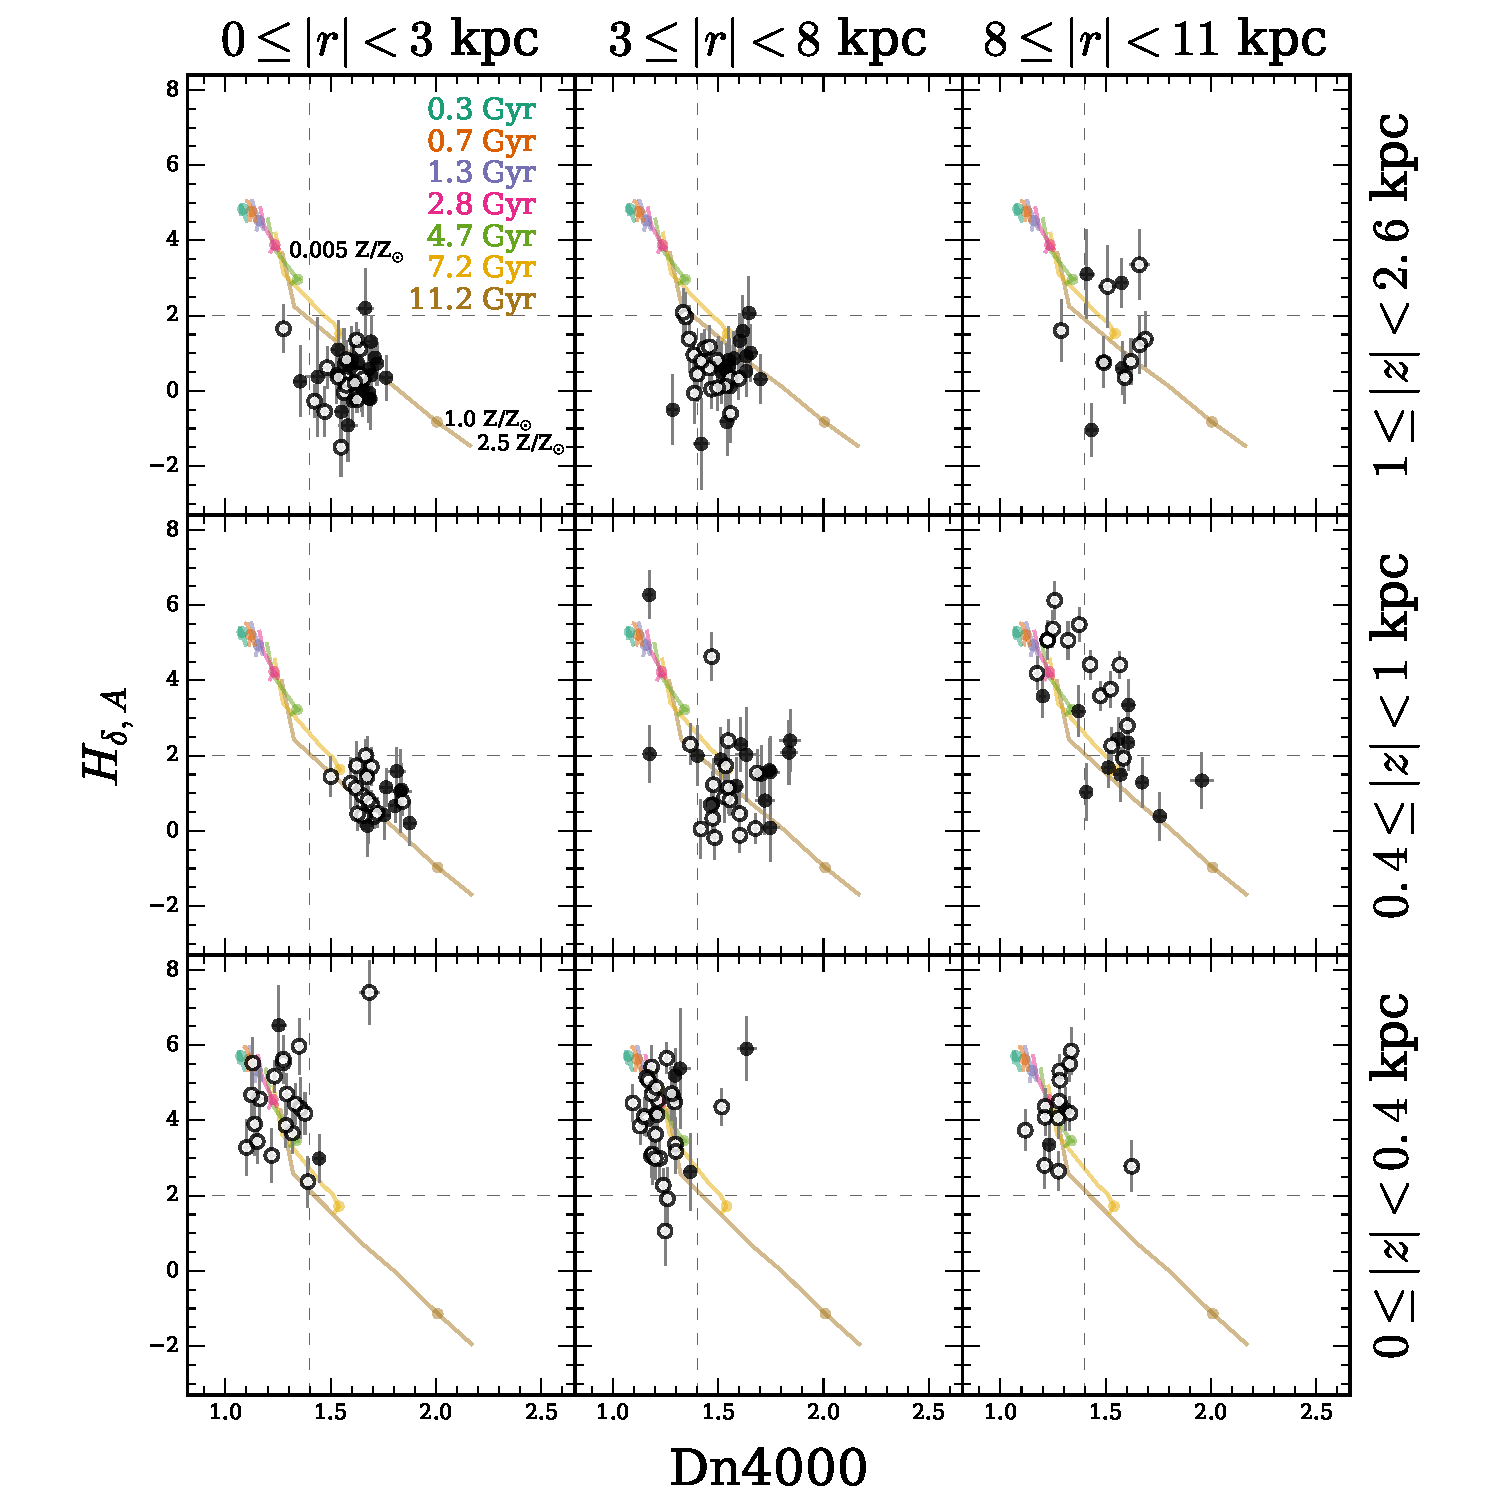
\includegraphics[width=0.8\textwidth]{891_1/figs/Dn4000_multires.pdf}
  \caption[$D_n(4000)$ vs \Hda in radius and height
  bins]{\label{891_1:fig:D4000_cuts}\fixspacing Spectral indices \Hda and
    $D_n(4000)$ for all good apertures in NGC 891 as a function of
    projected radius and height. Rationale for radial and vertical
    bins is provided in the text. Open symbols are for apertures on
    the approaching side, while filled circles are for apertures the
    receding side. Color-coded isochrones, labeled by their mean,
    light-weighted age at 5550 \AA\ are based on models with
    exponentially declining star-formation and a total age of 12 Gyr,
    as described in \S\ref{891_1:sec:fidgrid}; these are shown to
    highlight trends in age and the dependence of these indices on
    metallicity. The extreme values of metallicity are shown at the
    ends of the oldest isochrone in the top-left panel; solar
    metallicity for each isochrone is marked with a filled circle in
    all panels. The model values are adjusted for the mean
    instrumental resolution of each vertical bin as described in the
    text. Dashed lines are fiducial to highlight trends in age.}
\end{figure*}

We use \Hda and $D_n(4000)$ as our primary age indicators. As noted by
\citet{Hamilton85} these two indices are generally anti-correlated and
are useful, when combined, as an estimator of population age because
of their sensitivity to different star-formation time-scales.
Historically, \Hda has been used with $B-R$ color
\citep[e.g.,][]{Couch87} to discriminate between different
star-formation scenarios involving bursts, but \citet{Balogh99} has
shown that $D_n(4000)$ works as a suitable alternative to color, as
one might expect based on the correlations shown in
\citet{Hamilton85}. In essence, $D_n(4000)$ is a narrow-band color
intermediate in the wavelength range spanned by $U-B$. Because of its
relatively narrow band-pass it is more immune from extinction effects,
say, than broad-band colors.

Figure \ref{891_1:fig:D4000_cuts} shows these measurements grouped into
three radial and three vertical bins. The radial bins are chosen to
sample the region within the inner truncation of the super-thin disk
($|r| < \val{3}{kpc}$), the super-thin disk itself ($\val{3}{kpc}\leq
|r| < \val{8}{kpc}$), and beyond the outer super-thing disk truncation
($\val{8}{kpc} \leq |r|$) \citep{Schechtman-Rook13}. Vertical bins
were chosen to illustrate the stratification seen in stellar
populations: below \val{0.4}{kpc} stellar light is dominated by young
populations with strong Balmer absorption, but above this height we
see old populations with weak Balmer absorption and a correspondingly
strong $D_n(4000)$ break.

Again, as we saw in the comparison of Figures \ref{891_1:fig:MW_heating} and
\ref{891_1:fig:mab_data}, the results in Figure \ref{891_1:fig:D4000_cuts} for
the vertical age gradients are qualitatively consistent with the basic
heating model tuned to the MW solar cylinder presented in
\S\ref{891_1:sec:introduction}. Our MW heating model predicts this
transition to occur at roughly the scale-height of the old, thin
disk. The exact value depends on the assumed star-formation history
and how the scale-height is measured (e.g., band-pass and number of
components). We can begin by assuming the star-formation histories are
comparable for the two galaxies. In NGC 891 we find a sharp transition
from young to old stellar populations at \val{0.4}{kpc}. This is very
close to the vertical exponential scale-height for a single component
stellar disk fit to the broad-band light profile; \citet{Xilouris99}
find values of ranging from 0.34 to 0.43 kpc from the $K$ to $B$
bands, accounting for attenuation. For comparison, the super-thin and
thin disk components measured in the near-infrared $K$ band are 0.16
and 0.47 kpc, respectively. It is reasonable to presume that the
super-thin and thin components correspond to the young and old thin
disks in NGC 891.

Radial age gradients are minimal at low heights, but above the
midplane we see evidence for younger stars at larger radii,
particularly on the approaching side where there is an excess of
H$\alpha$, as discussed in Section \ref{891_1:891_1:sec:obs}. This gradient is
most pronounced for $\val{0.4}{kpc} \leq |z| < \val{1}{kpc}$ but is
visible even at the largest heights.

Discounting the azimuthal asymmetry for a moment (here projected onto
radius on either side of the center), this radial trend is indicative
of inside-out disk formation combined with disk flaring as seen in
simulations of MW-like disks \citep[e.g.,][]{Martig14a}. There is
ample evidence in today's massive disk galaxies that such a scenario
may indeed be viable. For example, in the MW and NGC 891 there is
evidence for gas flaring in atomic and molecular gas \citep[e.g.,][for
  NGC 891]{Scoville93, Yim11}. There also is recent evidence for
stellar flaring in the MW \citep{Ness16} as seen for age-dated giant
stars from APOGEE \citep{Majewski15}. In the $z\sim1$ galaxy
population there is also ample evidence of inside-out disk formation
based on Hubble Space Telescope studies \citep[e.g.,][]{Nelson15},
even for MW-like masses \citep[e.g.,][]{vanDokkum13}. This growth
pattern appears to be part of a broader trend (in time and galaxy
type) of size evolution \citep[e.g.,][]{Shibuya15}, although the
interpretation is challenging given the complexity of present day
mass-size relations seen, e.g., by \citet{Lange15} in the GAMA survey.
Nonetheless, spatially resolved spectroscopic maps of nearby galaxies
clearly show age gradients in disks, with the outer parts of disks
being younger in a light-weighted sense
\citep{Sanchez-Blazquez14,Gonzalez-Delgado15}. What we are able to
resolve here, for the first time in a massive spiral galaxy external
to the MW, is the {\it vertical} structure of these radial gradients.

Now considering the azimuthal asymmetry in star-formation and spiral
arm projection, it is clear that this asymmetry is reflected in the
vertical and radial gradients in the mean stellar age as reckoned in a
light-weighted sense with the indices in Figure \ref{891_1:fig:D4000_cuts}.
At the very least this should provide a cautionary reminder that
interpreting the radial and vertical gradients of spectral indices in
terms of specific scenarios (e.g., disk flaring and inside-out growth)
is necessary but perhaps not sufficient proof of the scenario's
plausibility. In particular, the role of projection, especially in the
context of the spiral arms and extinction, needs to be accounted for
as well \citep[cf the relative excess of H$\alpha$ vs 24$\mu$
  emission, as discussed in][]{Kamphuis07b}. We will show elsewhere
that differential SFH as a function of radius (where the outer
portions of disks are younger but not thicker) can also lead to {\it
  apparent} flaring in integrated star-light of a constant-thickness
disk. While star counts can certainly distinguish between flaring and
radially modulating SFH scenarios, for galaxies beyond the reach of
resolved stellar populations, stellar kinematics is likely the only
recourse to resolve different physical scenarios.

% see ALT TEXT above

% The radial gradients are consistent with an inside-out view of
% galaxy disk formation {\bf OG inside out ref}. Studies of high
% redshift galaxies \citep{Nelson12,Nelson13,Nelson15} {\bf we could
% go crazy with refs here} have shown that many disk galaxies exhibit
% a higher specific star formation rate and larger \Ha equivalent
% widths at large radii. This is often attributed to quenching in the
% inner regions caused by AGN and feedback after the initial burst of
% star formation, and there is evidence that is phenomenon is only
% observed in higher mass galaxies ($M_{\ast} > 10^{10.5}M_{\odot}$)
% \citep{Pan15,others?}. Regardless of whether these high-redshift
% disk are progenitors of disks at $z=0$ there is still evidence for
% similar trends in the local universe
% \citep{Sanchez-Blazquez07,Sanchez-Blazquez14} {\bf again, many more
% refs available}; disk galaxies show a larger proportion of young
% vs. old stars at larger radii, compared to the central regions.

The model grid in Figure \ref{891_1:fig:D4000_cuts} also highlights the
degeneracy between age and metallicity. Each colored line corresponds
to an isochrone of a given mean light-weighted age with varying values
of metallicity. As age increases the metallicity dependence in \Hda
and $D_n(4000)$ also increases. At an age of \val{\asim 11}{Gyr} these
indices can vary by almost the entire dynamic range of our data just
by assuming a different value for metallicity.  This age-metallicity
degeneracy is somewhat ameliorated by considering a reduced range of
metallicity (between 0.2 and 2.5 \Zsol), which we will show next is
plausible. Moreover, despite these degeneracies there is still a clear
distinction between ``young'' and ``old'' populations across the
vertical cut at \val{0.4}{kpc}; it is the actual age of this cutoff
that depends on metallicity.

\subsection{Metallicity and Abundance Gradients}
\begin{figure*}
  \centering
  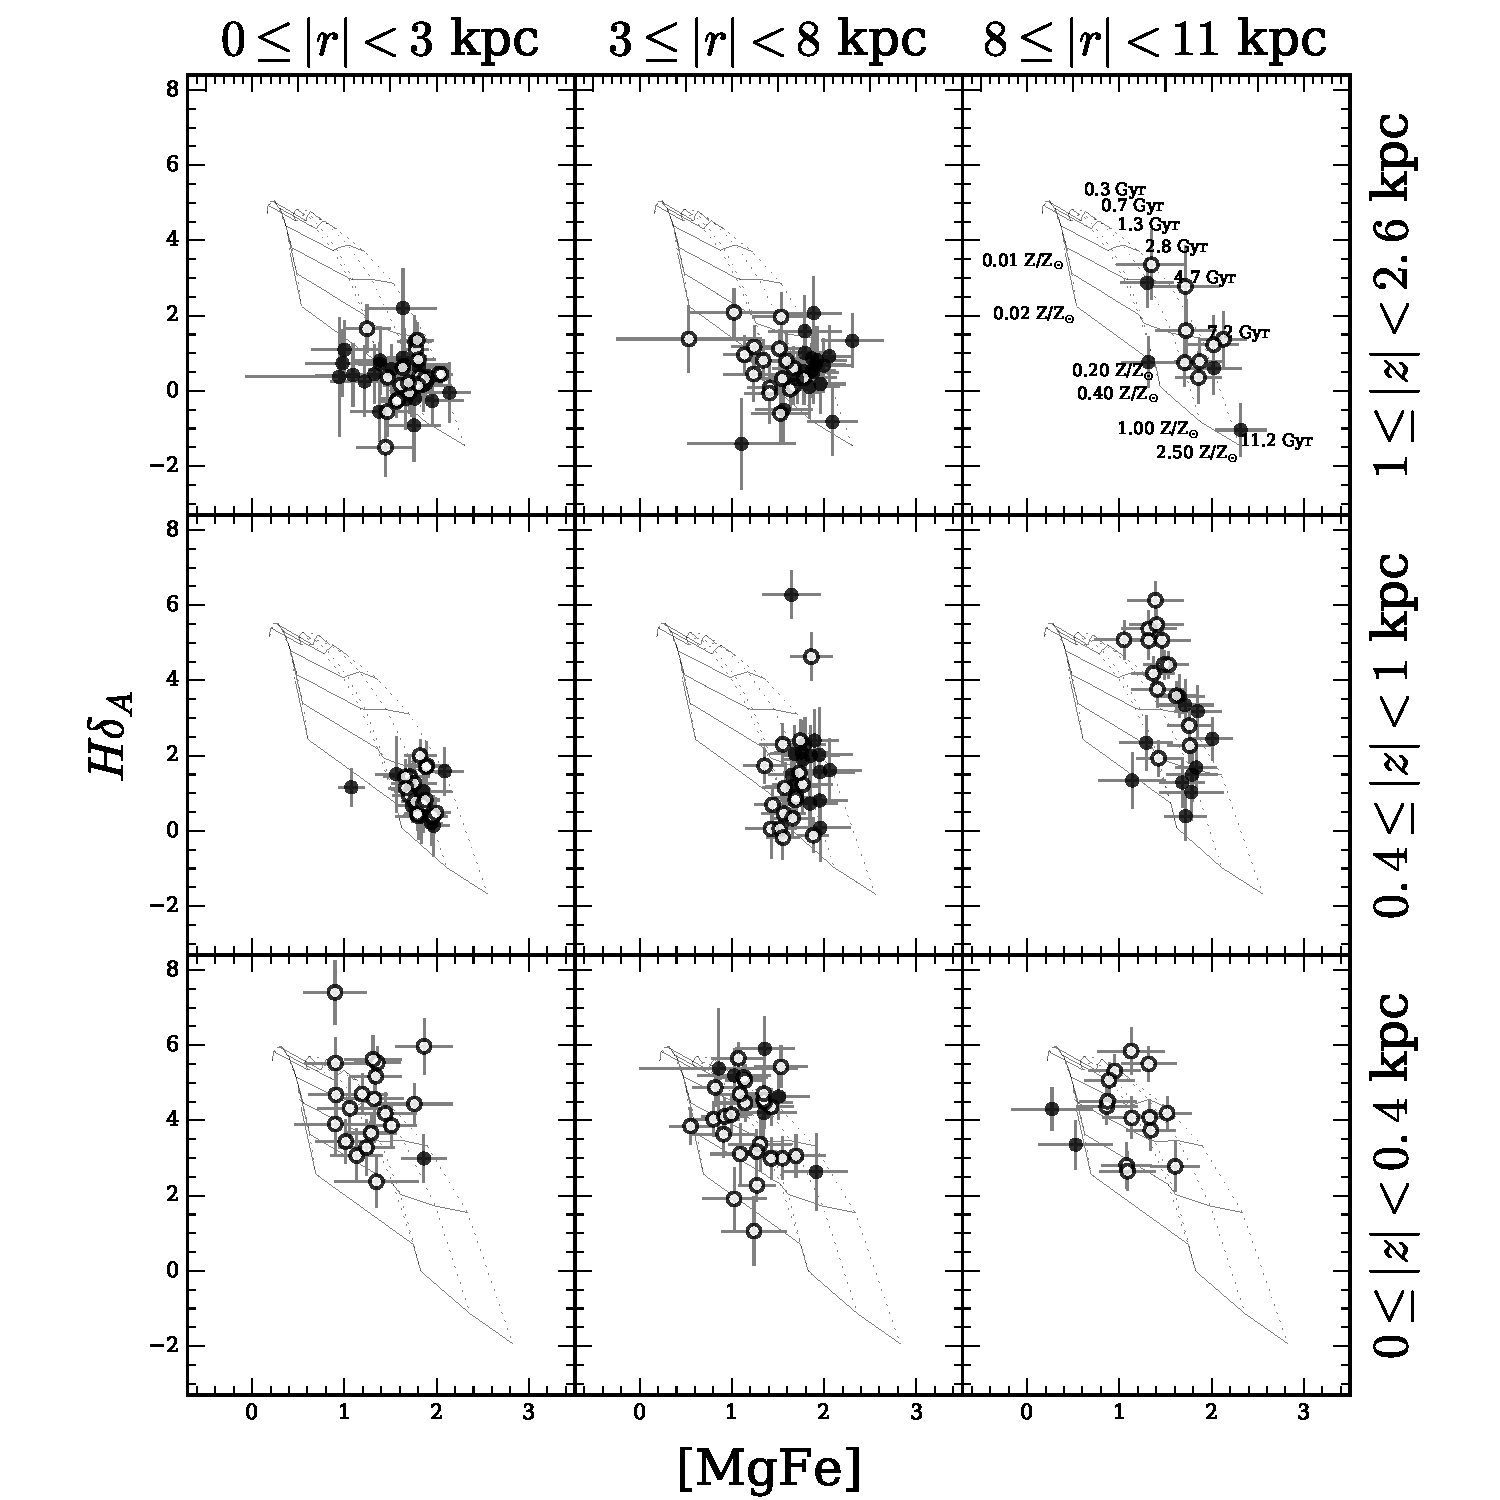
\includegraphics[width=0.8\textwidth]{891_1/figs/MgFe_multires.pdf}
  \caption[{[MgFe] vs \Hda in radius and height
    bins}]{\label{891_1:fig:MgFe_cuts}\fixspacing Spectral indices \Hda and
    [MgFe] for all apertures as a function of projected radius and
    height. Symbols, bins in radius and height, and models are the
    same as in Figure \ref{891_1:fig:D4000_cuts}. Lines of constant mean
    light-weighted age (isochrones, solid lines) and lines of constant
    metallicity (isofers, dotted lines) for the models are labeled in
    the top-right panel. The model values are adjusted for the mean
    instrumental resolution of each vertical bin as described in the
    text.}
\end{figure*}

Figure \ref{891_1:fig:MgFe_cuts} shows how metallicity (traced by [MgFe])
varies in the same bins defined in \S\ref{891_1:sec:age_grad} and Figure
\ref{891_1:fig:D4000_cuts}. Since [MgFe] is also age sensitive, we plot it
versus \Hda.  Guided by the fiducial grid described in
\S\ref{891_1:sec:fidgrid} we do not see significant trends in metallicity
with radius or height. The preponderance of apertures are well
described by metallicities in the range of $0.2 < Z/Z_\odot < 2.5$.

The lack of discernible gradients is perhaps unsurprising given the
precision of the measurements and the small dynamic range of the
indices, particularly for young ages. There are also line-of-sight
effects to consider as well. For example, there is a weak trend toward
slightly higher metallicities at intermediate heights. This may
appear counter-intuitive, but it may well reflect the confluence of
negative vertical and radial metallicity gradients and the fact that
as we move above the mid-plane the deprojected radii become smaller as
extinction diminishes.  In other words, all else being equal, young
formed near the center of a galaxy have higher metallicity than
young stars forming at large radii. Thus, at low heights where we
cannot see far into the disk we expect to find young populations with
low metallicity, but as height increases we can detect light from
smaller radii where the metallicity is on average higher.

While age gradients are again apparent in height Figure
\ref{891_1:fig:MgFe_cuts}, as too is the possible flaring of young stars
in the outer disk particularly on the approaching side, what is
also readily apparent is an asymmetry in the metallicity on the two
sides of the galaxy at intermediate radii. The receding side of the
galaxy, where there is less evidence for flaring, appears to be more
metal rich. This enhancement is most evident at intermediate and large
heights, i.e., for the older stars. This may also be a line-of-sight
depth effect in the sense that we are seeing farther in to the disk on
the receding side where, for a given height, metallicity is higher.

% We suspect our results stem from a combination of high optical depth
% at radial metallicity gradients. NGC 891 is known to be optically
% thick at optical wavelengths to heights of XXXX
% \citep{Xilouris99,Shcechtman-Rook12,?} so at low heights we can only
% observe populations at large radii. Furthermore, numerous studies of
% the Milky Way \citep{Hayden15,?,?} and external galaxies
% \citep{Ferguson98, vanZee98, ?} have shown that the metallicity of
% the ISM is anticorrelated with radius.
\begin{figure*}
  \centering
  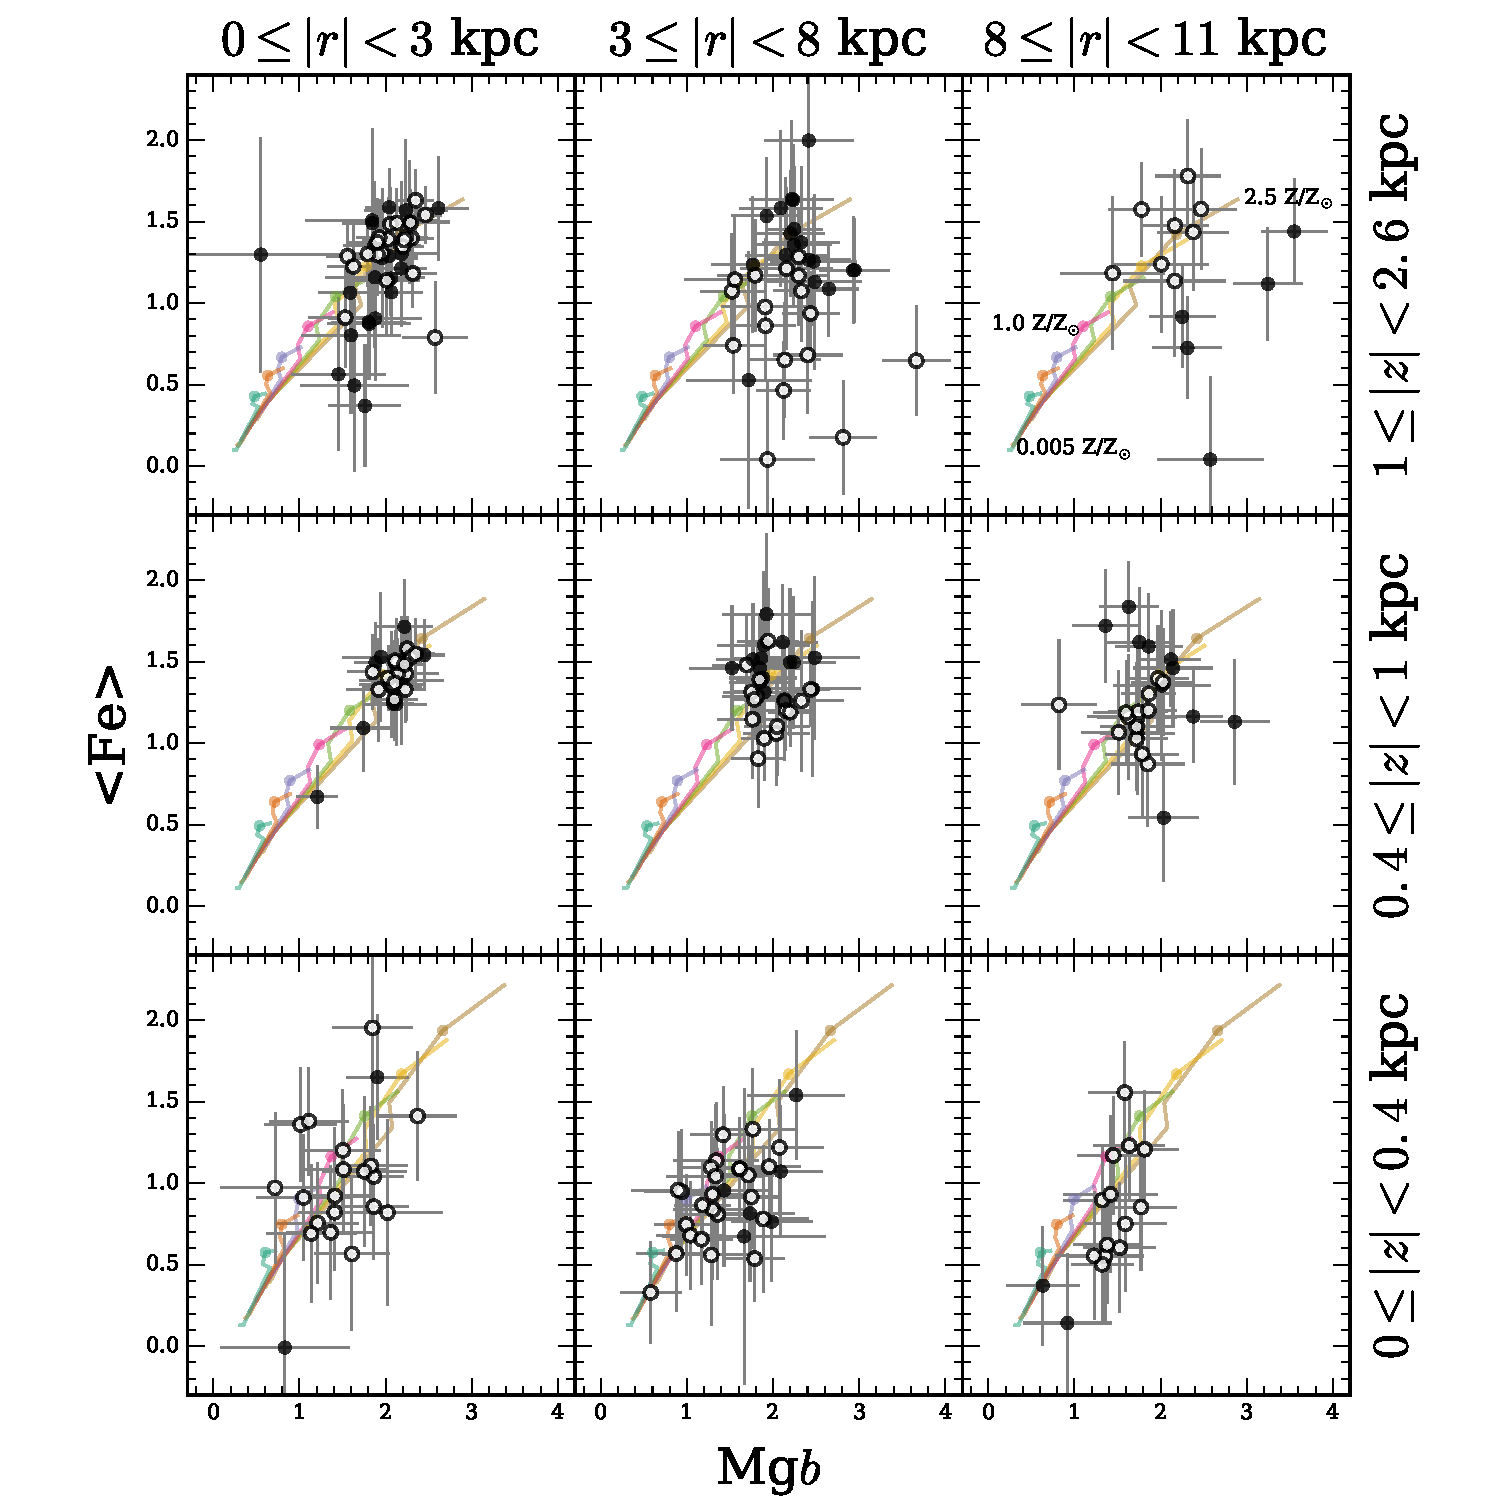
\includegraphics[width=0.8\textwidth]{891_1/figs/Mgb_multires.pdf}
  \caption[Mg$b$ vs $\left<\mathrm{Fe}\right>$ in radius and height
  bins]{\label{891_1:fig:Mgb_cuts}\fixspacing Spectral indices
    $\left<\mathrm{Fe}\right>$ and Mg$b$ for all apertures as a
    function of projected radius and height. Symbols, bins in radius
    and height, and model grid (including color-coding for age) are
    the same as in Figure \ref{891_1:fig:D4000_cuts}. The model values are
    adjusted for the mean instrumental resolution of each vertical bin
    as described in the text.}
\end{figure*}

In Figure \ref{891_1:fig:Mgb_cuts} we examine how abundance changes in our
data with radius and height. Based on the results of \citet{Thomas03}
(specifically their Figure 4) we note that populations with different
abundance will occupy different loci in the Mg$b$ vs
$\left<\mathrm{Fe}\right>$ plane, with higher abundance populations at
smaller values of $\left<\mathrm{Fe}\right>$ and slightly larger
values of Mg$b$. In general, increasing overall metallicity moves
points diagonally upward in this plot.

The differences in metallicity seen at intermediate radii and larger
heights in Figure \ref{891_1:fig:MgFe_cuts} appear to not have associated
abundance gradients.  There is some evidence for enhanced abundances
at low heights, and again at the largest heights. At intermediate
heights, where the errors are also the smallest, the abundances appear
to be very close to solar.

% The slope of the dashed lines in Figure \ref{fig:Mgb_cuts} is based on
% the distinction between high and low abundance models shown in
% \citet{Thomas03}.

%% The fiducial grid in this figure shows the Mg$b$ vs. <Fe>
%% plane is weakly sensitive to metallicity, but we caution that this
%% might be a result of a constant abundance {\bf WHAT IS IT?} across the
%% model galaxies used to construct it.
%% At low and intermediate heights
%% the abundance is remains constant while the age increases. Above
%% \val{1}{kpc}, however the age is relatively constant while the
%% abundance increases. This trend is especially prevelant at radii
%% beyond the inner portion of the galaxy.

% Below \val{1}{kpc} there is very little change in abundance with
% either radius or height, but above \val{1}{kpc} there is a clear
% transition to populations with a higher level of
% $\alpha$-enhancement. This is consistent with our claim of older
% populations at larger heights, but the fact that the transition in
% abundance occurs above the transition detected in Dn400 and \Hda
% indicates some mixing of populations between 0.4 and \val{1}{kpc}.

% Our conclusions that total metallicity and abundance respectively
% decrease and increase with height are generally consistent with
% detailed observations of the solar neighborhood
% \citep{Bovy12,Hayden15} and nearby galaxy disks
% \citep{Sanchez-Blazquez07}.

% \begin{figure*}
%   \centering
%   \includegraphics[width=\textwidth]{figs/index_height.pdf}
%   \caption{\label{fig:index_height}Each of the indices described in
%     \S\ref{891_1:sec:index_defn} plotted as a function of height above the
%     midplane. Vertical lines mark the borders of the vertical bins
%     shown in Figures \ref{fig:D4000_cuts} - \ref{fig:Mgb_cuts} and the
%     three radial bins used in the same figures are shown in different
%     colors. The transition from young to old populations at
%     \val{0.4}{kpc} is clear in the \Hda and $D_n4000$ panels. The three
%     lower panels show that abundance increases with height.}
% \end{figure*}
%
% [THIS IS THE TEXT THAT WENT WITH THE ABOVE FIGURE]
% Figure \ref{fig:index_height} shows the five indices measured above as
% a function of height above the midplane, where the transition from
% young to old populations is clearly visible at \val{0.4}{kpc} as
% measured in \Hda and $D_n4000$. Our primary abundance indicator,
% Mg$b$, also increases with height, but, interestingly, there is not as
% clear a break between high and low Mg$b$ values as there is with
% either $D_n4000$ or \Hda. However, coupled with a break to lower
% values of $\left<\mathrm{Fe}\right>$ above \val{1}{kpc} there is
% evidence of a high abundance population at these large heights,
% consistent with the results shown in Figure
% \ref{fig:Mgb_cuts}. Finally, we caution that, while it may appear the
% total metallicity increases with height, the [MgFe] index is highly
% dependent on age, as seen in Figure \ref{fig:MgFe_cuts}.

% \begin{figure*}
%   \centering
%   \includegraphics[width=\textwidth]{figs/repspec.pdf}
%   \caption{\label{fig:repspec}Binned spectra as a function of
%     projected radius and height. For each bin the spectrum is an
%     average of all apertures within the ($r,z$) limits shown, weighted
%     by the S/N of each aperture (see Table \ref{tab:data_ap}). At low
%     heights the spectra have strong \Hd absorption indicative of young
%     stellar populations, while larger heights show almost no \Hd
%     absorption but have a large break across \val{4000}{\AA}. The
%     results are qualitatively consistent with the heating referenced
%     in Figure \ref{fig:MW_heating}. Furthermore, at low heights there
%     is variation with radius, while at large heights the populations
%     seem to get slightly younger with increasing radius, perhaps
%     indicative of a flared disk.}
% \end{figure*}


